\documentclass[12pt,a4paper]{article}
  \usepackage[toc,page]{appendix}
  \usepackage{longtable}
  \usepackage{amsmath}
  \usepackage{booktabs}
  \usepackage{listings} 
  \usepackage{verbatim}
  \usepackage{graphicx}
  \usepackage{tabularx}
  \usepackage{subfig}
  \usepackage{float}
  \usepackage{multirow}
  \usepackage{pdfpages}
  \usepackage{csvsimple}
  \usepackage{hyperref}
  \usepackage[a4paper,bindingoffset=0.2in,left=0.6in,right=0.6in,top=1in,bottom=1in,footskip=.25in]{geometry}

  \usepackage{listings}
  \usepackage{color}
  \definecolor{white}{rgb}{0.95,0.95,0.95}
  \definecolor{darkgray}{rgb}{.1,.1,.1}
  \definecolor{purple}{rgb}{0.65, 0.12, 0.82}
  \definecolor{green}{rgb}{0,0.6,0}
  \definecolor{gray}{rgb}{0.5,0.5,0.5}
  \definecolor{main}{rgb}{0.06,0.34,0.41}

  \lstdefinelanguage{JavaScript}{
    keywords={typeof, new, true, false, catch, function, return, null, catch, switch, var, if, in, while, do, else, case, break},
    keywordstyle=\color{main}\bfseries,
    ndkeywords={class, export, boolean, throw, implements, import, this, from, default, it, renderer, create, expect, toMatchSnapshot, const, let, toEqual, simulate, shallow, find, exists, toBeTruthy, describe},
    ndkeywordstyle=\color{main}\bfseries,
    identifierstyle=\color{black},
    sensitive=false,
    comment=[l]{//},
    morecomment=[s]{/*}{*/},
    commentstyle=\color{purple}\ttfamily,
    stringstyle=\color{red}\ttfamily,
    morestring=[b]',
    morestring=[b]"
  }

  \lstset{
    language=JavaScript,
    backgroundcolor=\color{white},   % choose the background color
    basicstyle=\footnotesize,        % size of fonts used for the code
    breaklines=true,                 % automatic line breaking only at whitespace
    captionpos=b,                    % sets the caption-position to bottom
    commentstyle=\color{green},      % comment style
    escapeinside={\%*}{*)},          % if you want to add LaTeX within your code
    keywordstyle=\color{blue},       % keyword style
    stringstyle=\color{darkgray},     % string literal style
  }

  \hypersetup{%
    pdfborder = {0 0 0}
  }

  \begin{document}
    \begin{titlepage}
      \centering
      {\scshape\LARGE Goldsmiths, University of London \par}
      \vspace{1cm}
      {\scshape\Large Software project final report\par}
      \vspace{1.5cm}
      {\huge\bfseries iLost\par}
      \vspace{2cm}
      {\Large\itshape 
        Ahmed, Muhammad\\
        Chowdhury, Thairan\\
        Davies Minta, Dylan\\     
        Fakrul, Mahmudul\\    
        Farkhani, Hussein\\ 
        Jheng-Hao, Lin\\
        Pecorella, Mariano\\ \par}
      \vfill
      supervised by\par
      \textsc{Tim Blackwell} 
      \vfill
      % Bottom of the page
      {\large \today \par}
    \end{titlepage}
    \tableofcontents
    \newpage
    \section{Introduction}
      \paragraph{} Losing belongings is a common problem, roughly £70 worth of items are lost in the public per year. \textsuperscript{[1]} We conducted a survey about lost items to find out if we could create a useful application based on this concern. Following our survey, this statement was found to relate to university students as 89\% of our participants claimed to be susceptible to losing items. This information motivated us to reduce the loss of personal belongings; leading to the development of an item tracking application and a portable tracking device. Our app aims to circumvent the loss of bags and other valuables. The user will attach the portable tracker to their bag or belonging, allowing it to be tracked using our app. The app will notify the user when the distance between the app and tracker reaches 30m.
      

      This report will cover five main categories:

      \begin{itemize}
        \item {Development Record}:
          We explain the methodology used by our group to decide the technology with which to implement the app’s functionality alongside the development methods that were used. We also describe the way that the development was handled by the team and provide a reflection on its efficiency.

        \item {Formative Evaluation}:
          This section of the report describes our assessment with users during development. The formative evaluation details what we did during user testing and its outcomes.

        \item { Design and Implementation}:
          An overview of our final design and implementation, including any changes from our initial ideas with justifications for the significant decisions we made.

        \item { Quality Assurance}:
          We detail our approach to Quality Assurance and the testing carried out, including our results. An assessment of how well our final system imitates our initial requirements with justifications of any changes we made to the requirements.

        \item { Summative Evaluation}:
          A descriptive evaluation of the methods, results and conclusion of our final software.
      \end{itemize}

    \section{Development Record}
      \subsection{Teams} 
        % 400 - 500 words
        \paragraph{}During the implementation stage, we set up an organisation {\bf GSoft} on GitHub. We were divided into three teams, {\bf iOS app}, {\bf Android app} and {\bf Backend/Tracker team}, which shows in figure \ref{fig:Development Teams}. Each team was grouped by 2 to 3 people who were more interested in that topic or technology. Some of us were interested in more than two areas, if this was the case; members could join more then one team. The list of the team members can be found in table \ref{table:Teams}.
        \begin{figure}[H]
          \centering
          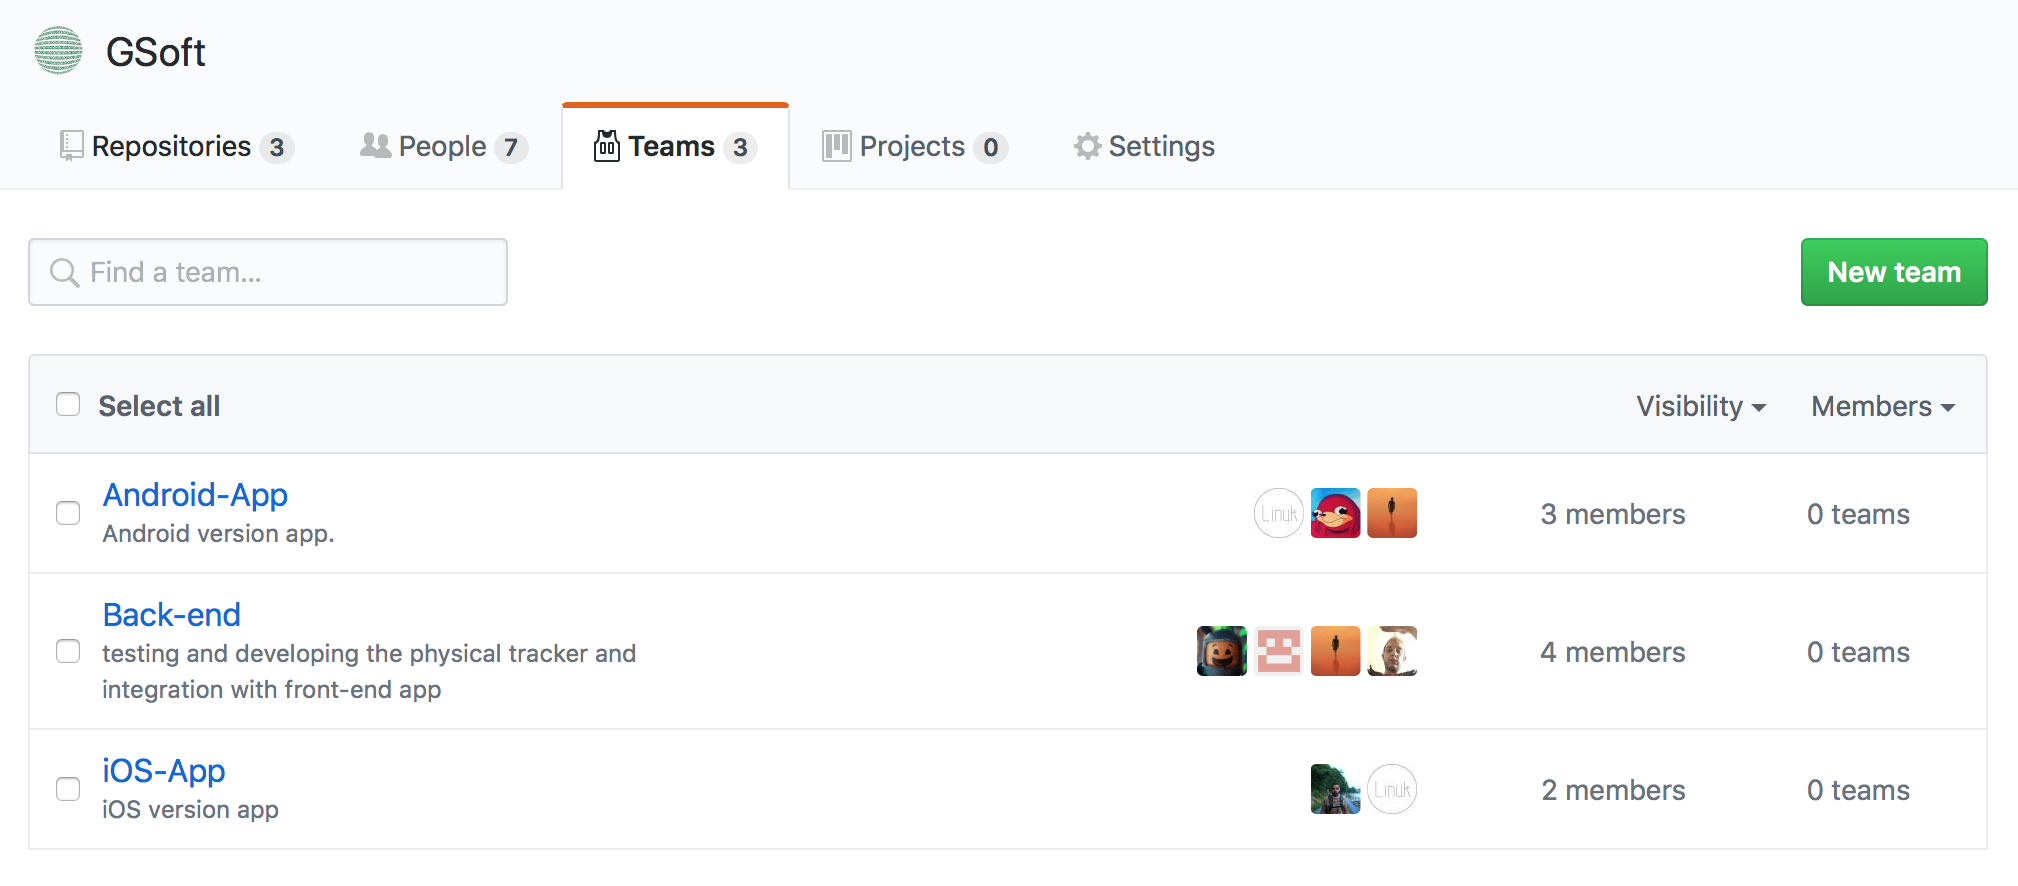
\includegraphics[width=1\textwidth]{../assets/development-records-teams.png}
          \caption{Development Teams on Github}
          \label{fig:Development Teams}
        \end{figure}

        \begin{table}[H]
          \centering
            \begin{tabularx}{\textwidth}{l X}
              \hline
               Team & Members \\ \hline
               iOS app & Jheng-Hao(leader), Muhammad \\
               Android app & Dyland(leader), Mahmudul, Jheng-Hao \\ 
               Backend/Tracker  & Hussein(leader), Thairan, Mahmudul, Mariano \\
              \hline
            \end{tabularx}
            \caption[Table caption text]{Teams}
            \label{table:Teams}
        \end{table}        

      \subsection{Technology Selection} 

        \paragraph{}Development Teams: Each team was responsible for how and what technology to use, as long as the production could be made on time. We believed this methodology had these advantages in terms of the limited development time:

        \begin{itemize}
          \item {React Agilely}: Compared to having a poll with all members of our group, it was agiler to come to the decision within 2 or 3 in their designated team. Since each team could react to the situation and resolve any issues in a more efficient way.
          \item {Specialities differ}: Our group was divided by our interests and specialities, we trusted each team could make the best decision for the whole team with their research and experience. For example, the iOS app team would not interfere with how the tracker team implemented the physical components at all; And how the Android app was implemented would not be the backend/tracker team's concern. All teams were trusted in which they would make the best decisions.
        \end{itemize}
        
        \paragraph{}Even though the team was separated, it was important to keep everyone on the same page. So each technological decision or propose was documented as an architecture decision record(ADR), which enabled us to have an overview of all the technological changes. According to Michael Nygard, each ADR contains five columns\cite{ArchitectureDecisionRecord}: 

        \begin{itemize}
          \item Title: A brief description of the idea proposed.
          \item Context: {\bf Why} do we need to make the decision or change.                   
          \item Decision: {\bf What} are the responses toward the decision.
          \item Status: {\bf Current} status of the decision which, should be {\bf accepted}, {\bf rejected} or {\bf deprecated}.
          \item Consequences: {\bf What} has become better or worse because of the decision.
        \end{itemize}

        Please find more, complete architecture decision records in \ref{appendix:Architecture Decision Records}.
        
        To make sure that the whole group had the latest information; We used several channels on Slack to keep everyone updated. Such as the {\bf iOS channel} was the place containing all updates related to the iOS application development, this is shown in figure \ref{fig:Slack iOS Channel}. 
        
        \begin{figure}[H]
          \centering
          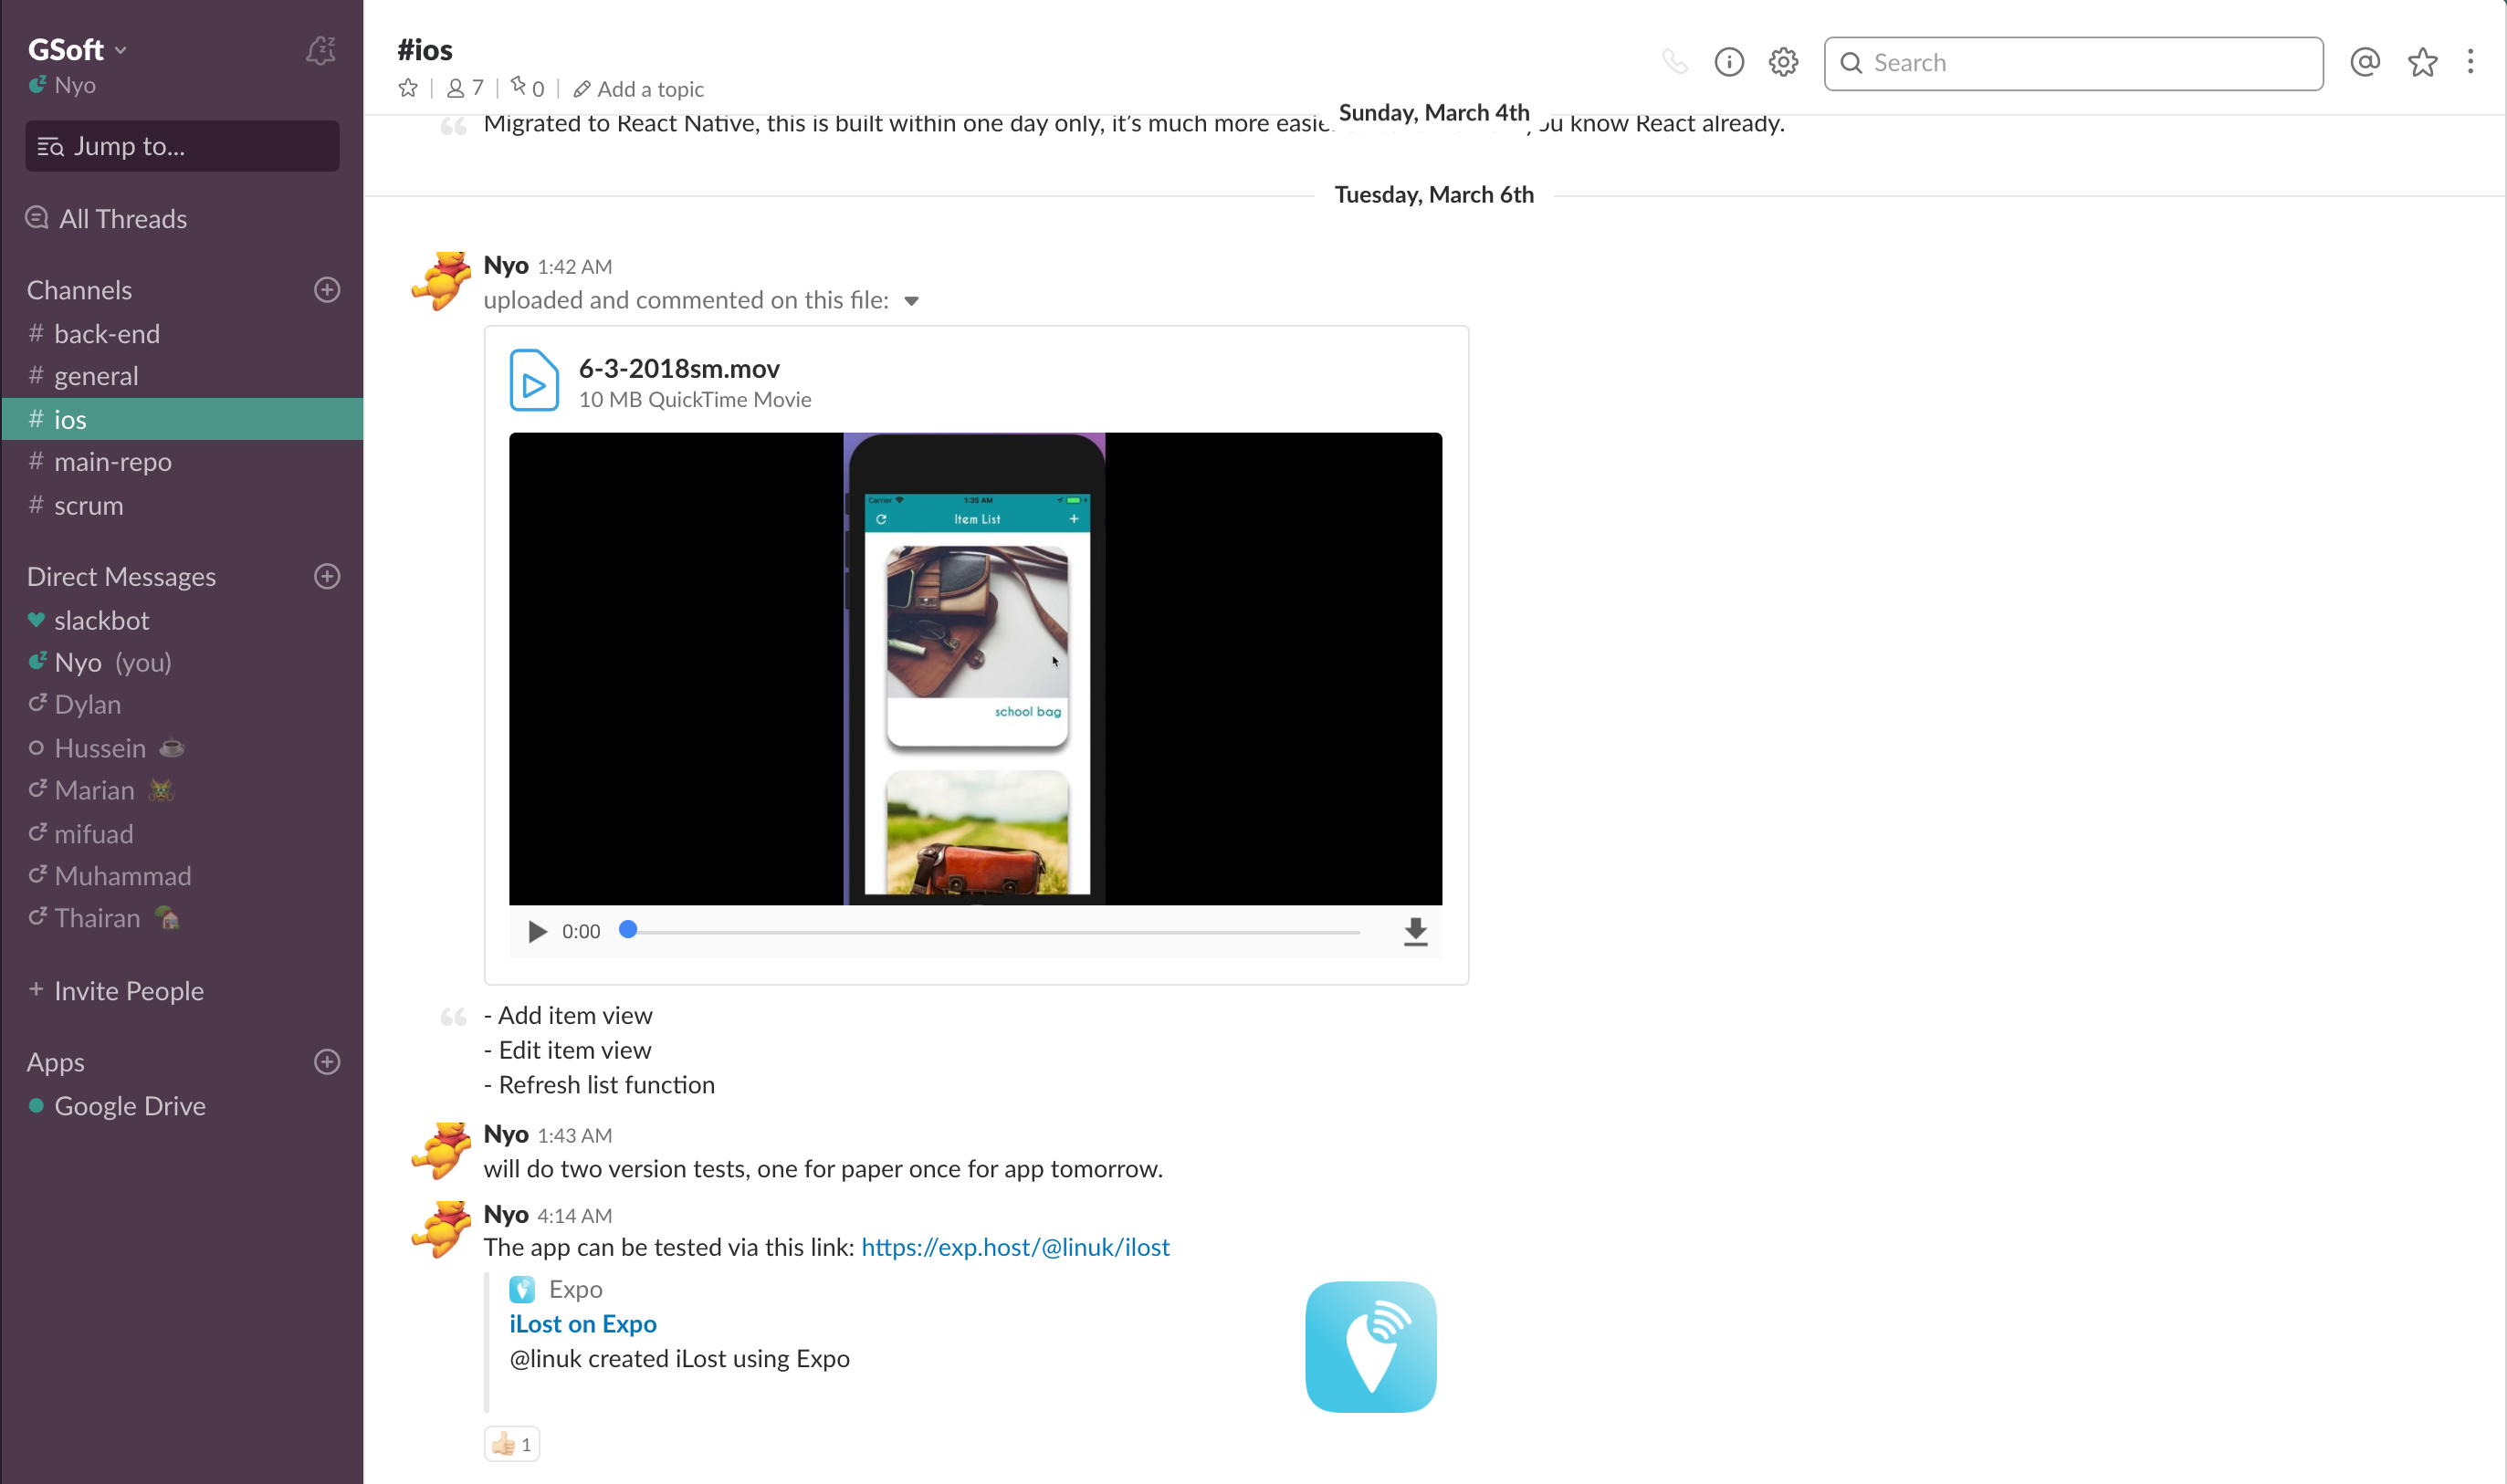
\includegraphics[width=1\textwidth]{../assets/development-records-slack-ios-channel.png}
          \caption{Slack iOS Channel}
          \label{fig:Slack iOS Channel}
        \end{figure}

      \subsection{Agile Development} 
        
        \paragraph{}Our team tried out two agile development methodologies, {\bf Scrum} and {\bf Kanban}.

        \subsubsection{Scrum Development}
          \paragraph{}Since we could not actually devote all of our time to develop the application, it would not be reasonable to do the daily scrum and have a meeting day-to-day for all of us. So in the beginning, we tried to set up a routine to simulate the daily scrum with Slack.

          \paragraph{}We defined 3 days per week for sprint sections to take place and whenever a sprint was finished, the team needed to answer three questions in the Scrum channel on Slack:
          
          \begin{itemize}
            \item What did I complete last time that it contributed to the team meeting our sprint goal?
            \item What do I plan to complete this time to contribute to the team meeting our sprint goal?
            \item Do I see any impediment that could prevent the team or me from meeting our sprint goal?
          \end{itemize}    

          \paragraph{}Unfortunately, not every team could follow the sprint process and make any progress every three days. Sometimes a team might work for a sprint then stopped for two sprints since other modules might have a deadline or coursework. Hence, this scrum process was not actually conducted properly and stopped after few weeks after started. The example records show in figure \ref{fig:Slack Scrum Channel}. 

          \begin{figure}[H]
            \centering
            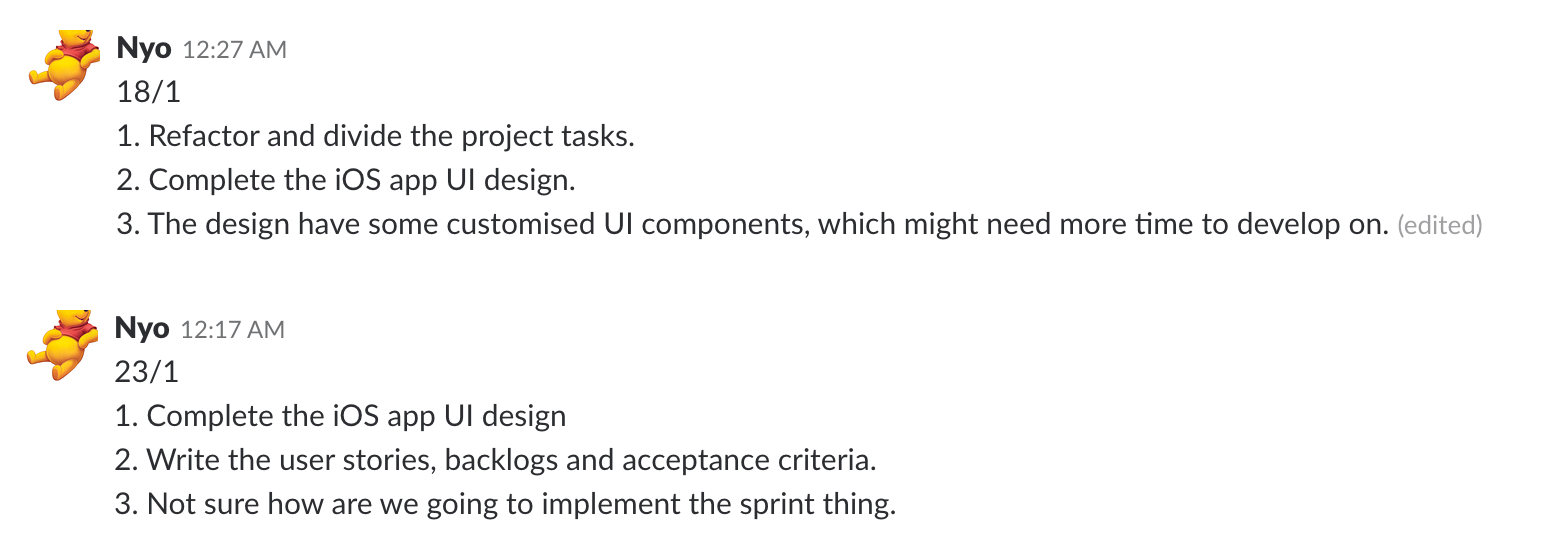
\includegraphics[width=1\textwidth]{../assets/development-records-slack-scrum-channel.png}
            \caption{Slack Scrum Channel}
            \label{fig:Slack Scrum Channel}
          \end{figure}
          
          \paragraph{}At the middle of the development stage, our supervisor suggested us to meet 2 hours a day and 2 to 4 days a week, work and team and engage the team building, since the progress tracking form showed that the working hours were really unbalanced and some people apparently did not put enough effort into the project. 
          
          \paragraph{}We made a daily sprint schedule, shown in figure \ref{fig:Daily Sprint} and followed by the time to do work together. Everyone should follow the schedule and spend at least two days a week to work together as a team. It went well and most of us were able to follow the schedule. We worked in RHB306a, 35 Cafe or the Whitehead building lab. But since the strike started, the daily sprint stopped again because not all of us were coming to the campus due to the long distance between home and the university. 

          \begin{figure}[H]
            \centering
            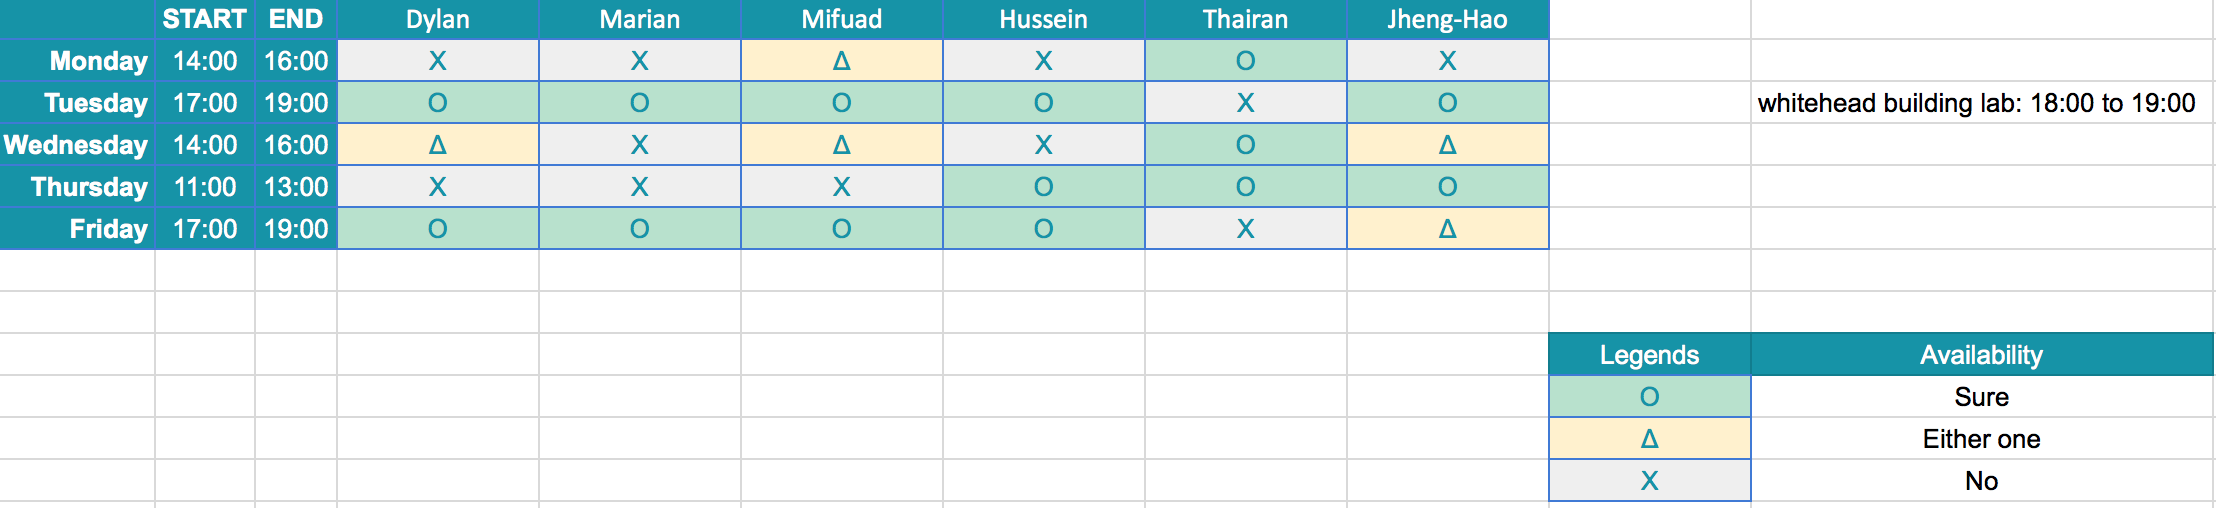
\includegraphics[width=1\textwidth]{../assets/development-records-daily-sprint.png}
            \caption{Daily Sprint}
            \label{fig:Daily Sprint}
          \end{figure}

        \subsubsection{Kanban}
          \paragraph{}Apart from the Scrum, Kanban was also implemented with the backlogs in our development to demonstrate the development progress. We tried to keep our project management tool simple and easy to approach, so we not only used GitHub for version control but also for the project feature, which we used it as the Kanban. The iOS  development Kanban was shown in \ref{fig:iOS Development Kanban}.

          \begin{figure}[H]
            \centering
            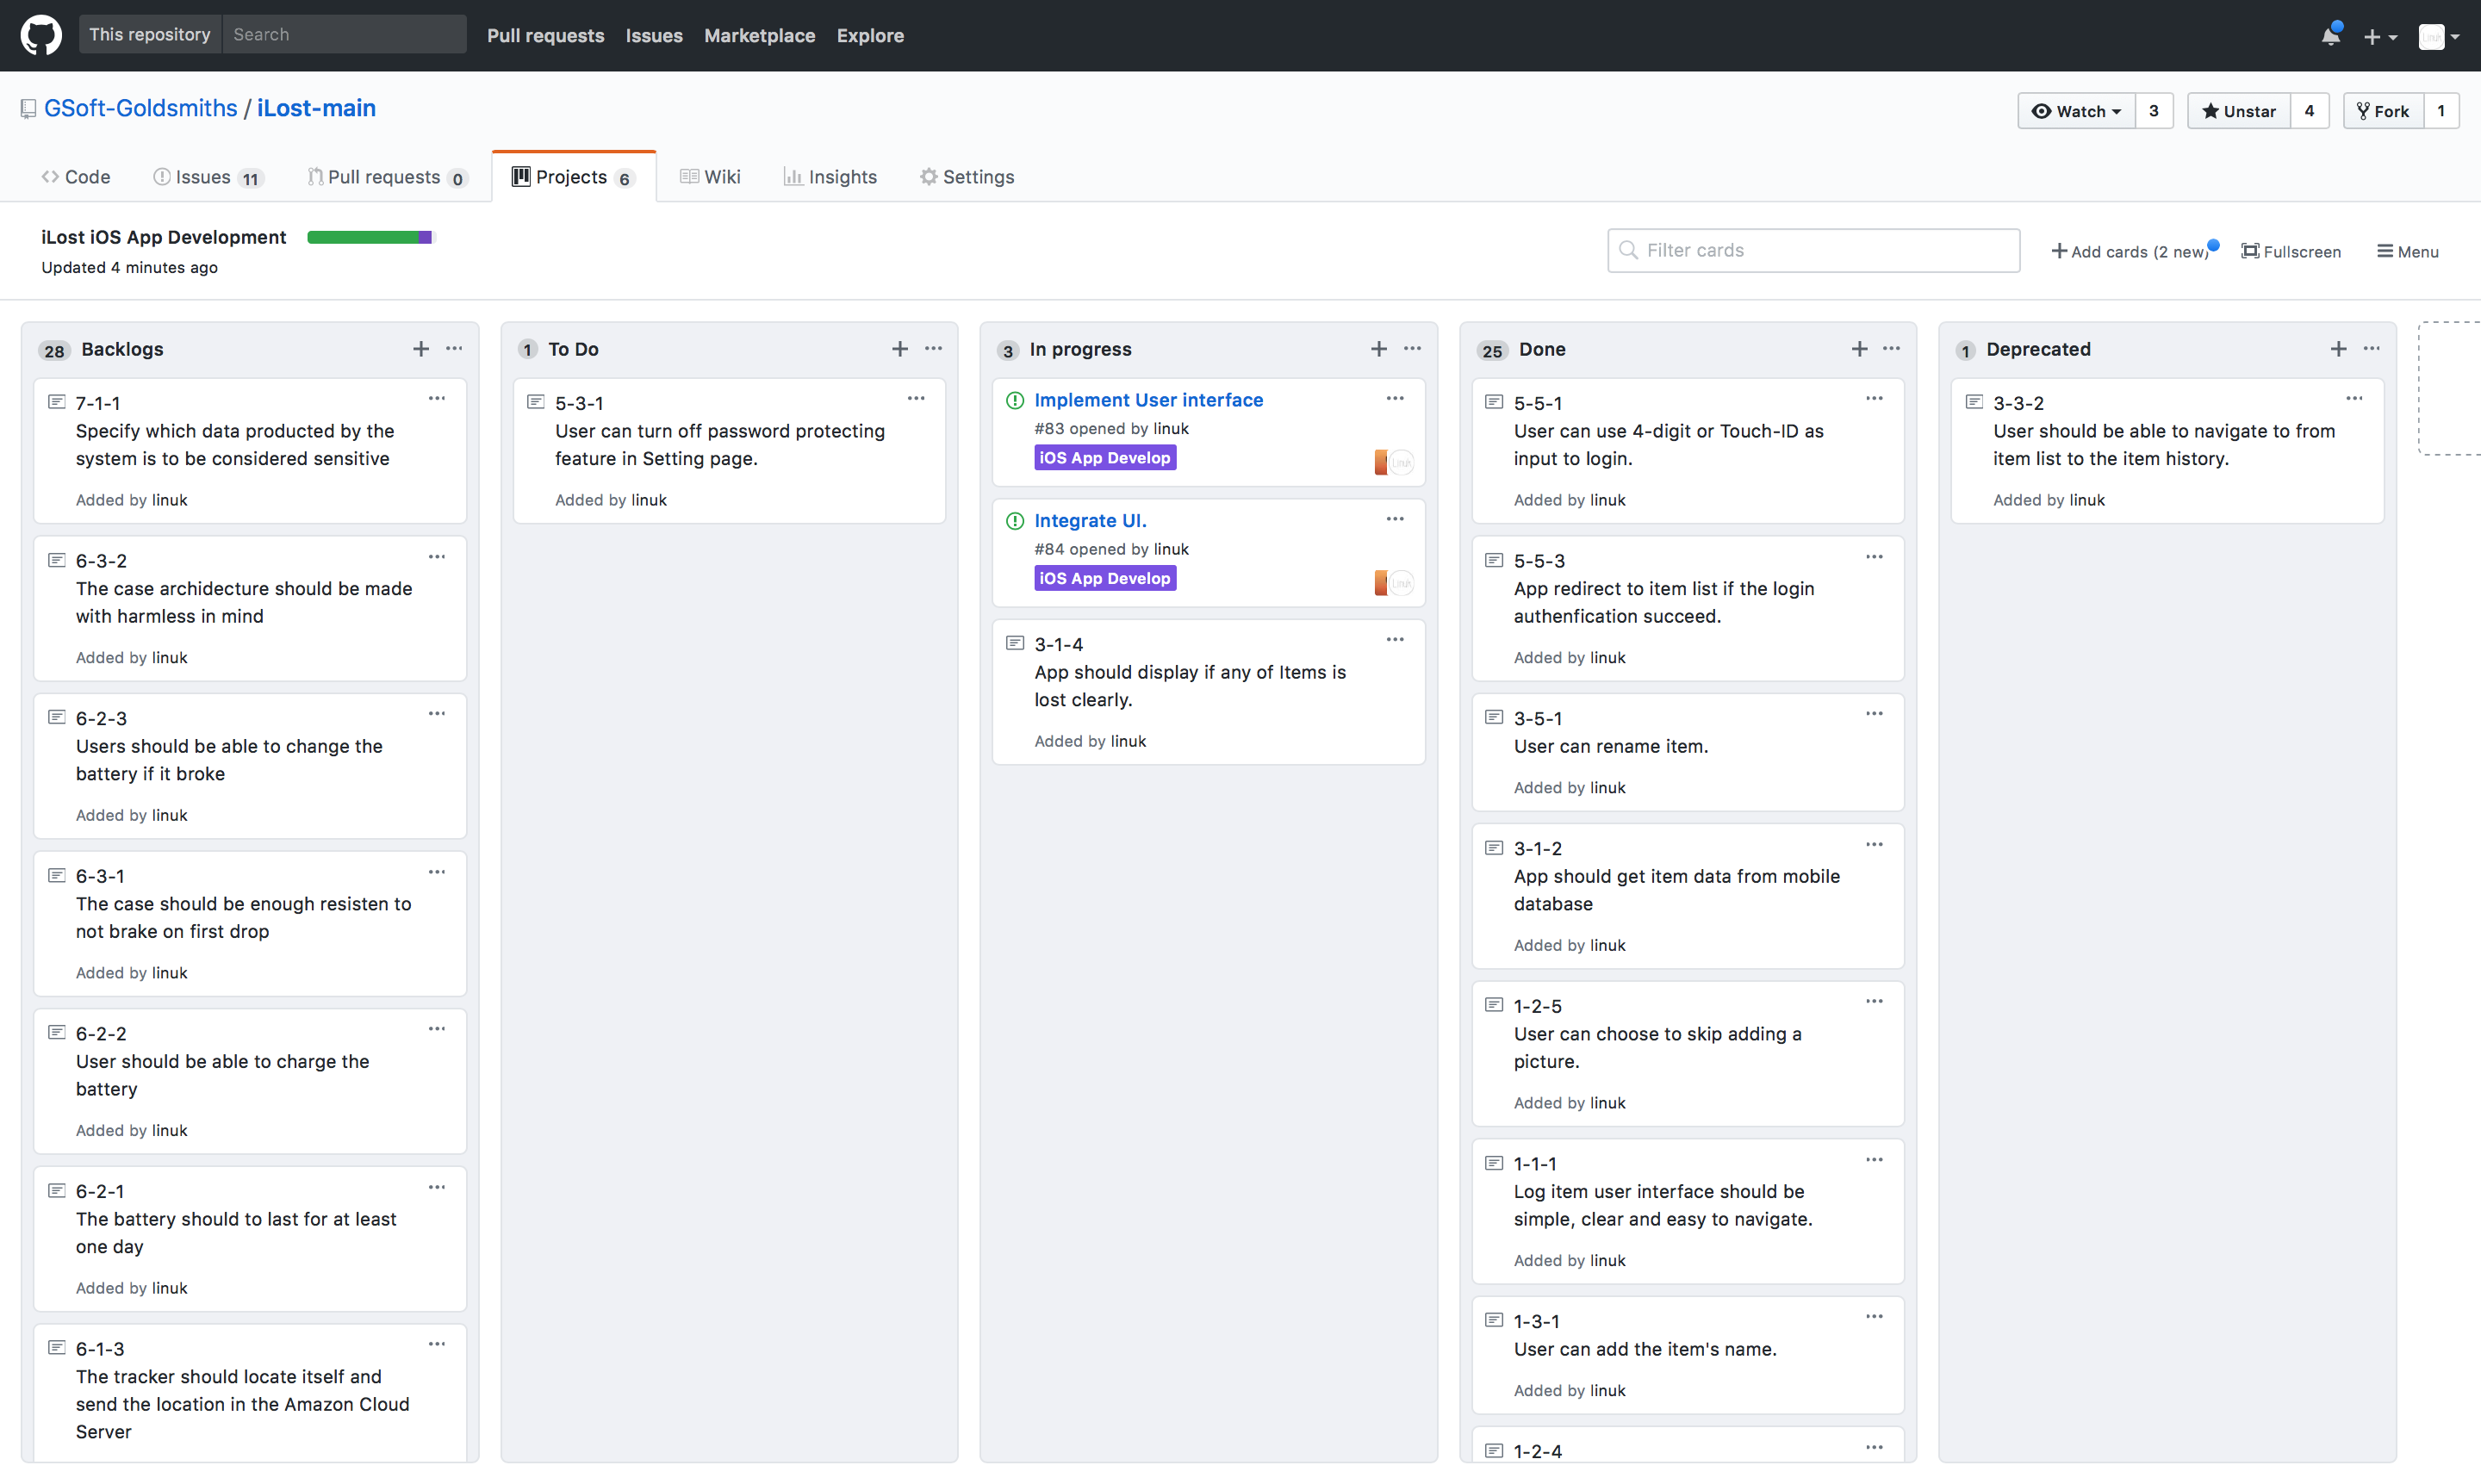
\includegraphics[width=1\textwidth]{../assets/development-records-ios-kanban.png}
            \caption{iOS app Kanban}
            \label{fig:iOS Development Kanban}
          \end{figure}
         
          Our Kanban contained five columns which shows in Table \ref{table:Kanban Columns}:
          
          \begin{table}[H]
            \centering
              \begin{tabularx}{\textwidth}{l X}
                \hline
                Column & Description  \\ \hline
                Backlogs & The task is scheduled to be developed, but it is possible to be assigned deprecated if it is no longer needed. \\ 
                To Do & The task is going to be developed.  \\ 
                In Progress & The task is currently developing.  \\ 
                Done & The task has been completed.   \\ 
                Deprecated & The task no longer needs to be developed.\\                  
                \hline
              \end{tabularx}
              \caption[Table caption text]{Kanban Columns}
              \label{table:Kanban Columns}
          \end{table}
          
          Apart from the normal columns: To Do, In Progress and Done, we also added {\bf Deprecated} to store the features or tasks that did not fit the needs anymore. Kanban gave a nice and clean overview of the current developing process, especially for people from other teams.
        
        \subsubsection{Behavior Driven Development}
          \paragraph{}In order to produce the minimum viable product(MVP), we followed the Behavior Driven Development(BDD) to develop our product. To implement this methodology, we wrote the backlogs of requirements specification at the beginning of the development stage. These requirements provided us with an overview of what was more urgent in what stage. 

          \paragraph{}For example, displaying the item's position and historical locations was one of the most important functionality, so its' priority was {\bf Must} and needed to be finished at the {\bf MVP} stage. On the other hand, navigating to the item by triggering Google Maps was helpful but might take longer to develop, so the priority was {\bf Should} and it should be developed at the {\bf Final} stage. 
          
          \paragraph{}Here was our development process of BDD:
          
          \paragraph{1. Requirements specification}Review the backlogs and pick one from them to work on based on the priority and the estimated development time. You can find the details of the backlogs in section \ref{section:Development Process - Backlogs}, Development Process - Backlogs.
          
          \paragraph{2. Design}Review the how was the data storage, data flow and the user interface design, then design how should this requirement be fulfilled. Such as displaying the item list in the item list view, we would need to implement two view components, an item list cell view and an item list table view. The item's properties data, including items id, name and photo, would be stored in the table view's state and the list cell would receive the props from the table view and render the item's properties.
          
          \paragraph{3. Development}Put the design into actual codes.
          
          \paragraph{4. Integration}Integrate the new view component with previously developed view components. Such as connecting the item list view with the item details view, where users could see its' location with a map.
          
          \paragraph{5. QA reviews}Conduct the quality assurance of the functionalities of latest and previously developed components. Please find more details in chapter \ref{chapter:Quality Assurance}, Quality Assurance.
          
          \paragraph{6. Usability tests}After several developments, we would bundle them as a new version of our mobile application. Then do the usability tests to test if any of the components, user interface or user experience could be improved. Please find more details in chapter \ref{Chapter:Formative Evaluation}, Formative Evaluation.
          
          \paragraph{7. Maintenance}After the usability tests, we did some improvements based on the usability testing results. 
          
          \paragraph{}This was a cycle process, after step 7 we went back to step 1 and kept going.

      \subsection{Development Process}
        \subsubsection{Backlogs}
          \label{section:Development Process - Backlogs}
          \paragraph{}Based on the user stories we made in the proposal, not only did we add more but also wrote sub-user stories and acceptance criteria's for each of them. We had a list contain backlogs stored in Google SpreadSheet, which contained these columns: 

          \begin{table}[H]
            \centering
              \begin{tabularx}{\textwidth}{l X}
                \hline
                Column & Description  \\ \hline
                User Story ID & The user story ID or sub-user story ID, a user story ID should be 1, 2, 3...n, and sub-user story should be 1-1, 1-2, 1-3, ... 1-m  where 1 is the parent user story.\\ 
                User Story & A brief description of the user story, starting with "As a user I want to ..." to describe what are the users' needs. Then followed by "so that ..." to explain why users need it. \\ 
                Backlog ID & An ID number for the backlog, a sub-user story may contain more than one backlog to satisfy the sub-user story. If a sub-user story ID is  3-5, then the task ID will be 3-5-1, 3-5-2, 3-5-3, ... 3-5-p.  \\ 
                Acceptance Criteria & A description of the backlog which describes how the mobile application or the tracker would satisfy the user stories. \\ 
                Priority & The priority of this backlog, should be {\bf Must}, {\bf Should} or {\bf Could}. \\                  
                Dev Days & The estimated developing times in days, 8 hours counted as one day. \\                  
                Phase & In which phase should the backlog be finished, in our case was either the {\bf MVP} or {\bf Final}. \\                  
                Process & The current developing process, which should be {\bf To Do}, {\bf In Progress}, {\bf Deprecated} or {\bf Done}.  \\                  
                \hline
              \end{tabularx}
              \caption[Table caption text]{Backlogs Columns}
              \label{table:Backlogs Column}
          \end{table}
          
          For example, the user story 3, {\bf Track Item: User uses App to see the tracking list and track Item.} This section has 7 sub-user stories, which shows in table \ref{table:Backlog Example: User Story 3}: 
          
          \begin{table}[H]
            \centering
              \begin{tabularx}{\textwidth}{l X}
                \hline
                 User Story ID & User Story \\ \hline
                 3-1 & As a user, I want to view the tracking item list so that I can view my item and look up more details if I want. \\
                 3-2 & As a user, I want to activate or deactivate the tracker so that I can save my mobile and the tracker's batteries. \\
                 3-3 & As a user, I want to see the location history in a map format of the item so that I can track/look for it, if it's lost. \\
                 3-4 & As a user, I want to navigate me to my item so that find it quicker. \\
                 3-5 & As a user, I want to edit my item's details so that I can change the tracking item. \\
                 3-6 & As a user, I want to delete the item so that I can stop tracking the item for good. \\
                \hline
              \end{tabularx}
              \caption[Table caption text]{Backlog Example: User Story 3}
              \label{table:Backlog Example: User Story 3}
          \end{table}   
          
          Take sub-user story 3-1 as an example. In order to satisfy this user story, we had 4 backlogs and acceptance criteria's to meet the requirements. Each of them had their own priority, estimated development days, phase and process. So this backlog will look like figure \ref{fig:Backlog Example: Sub-user story 3-1}:
          
          \begin{figure}[H]
            \centering
            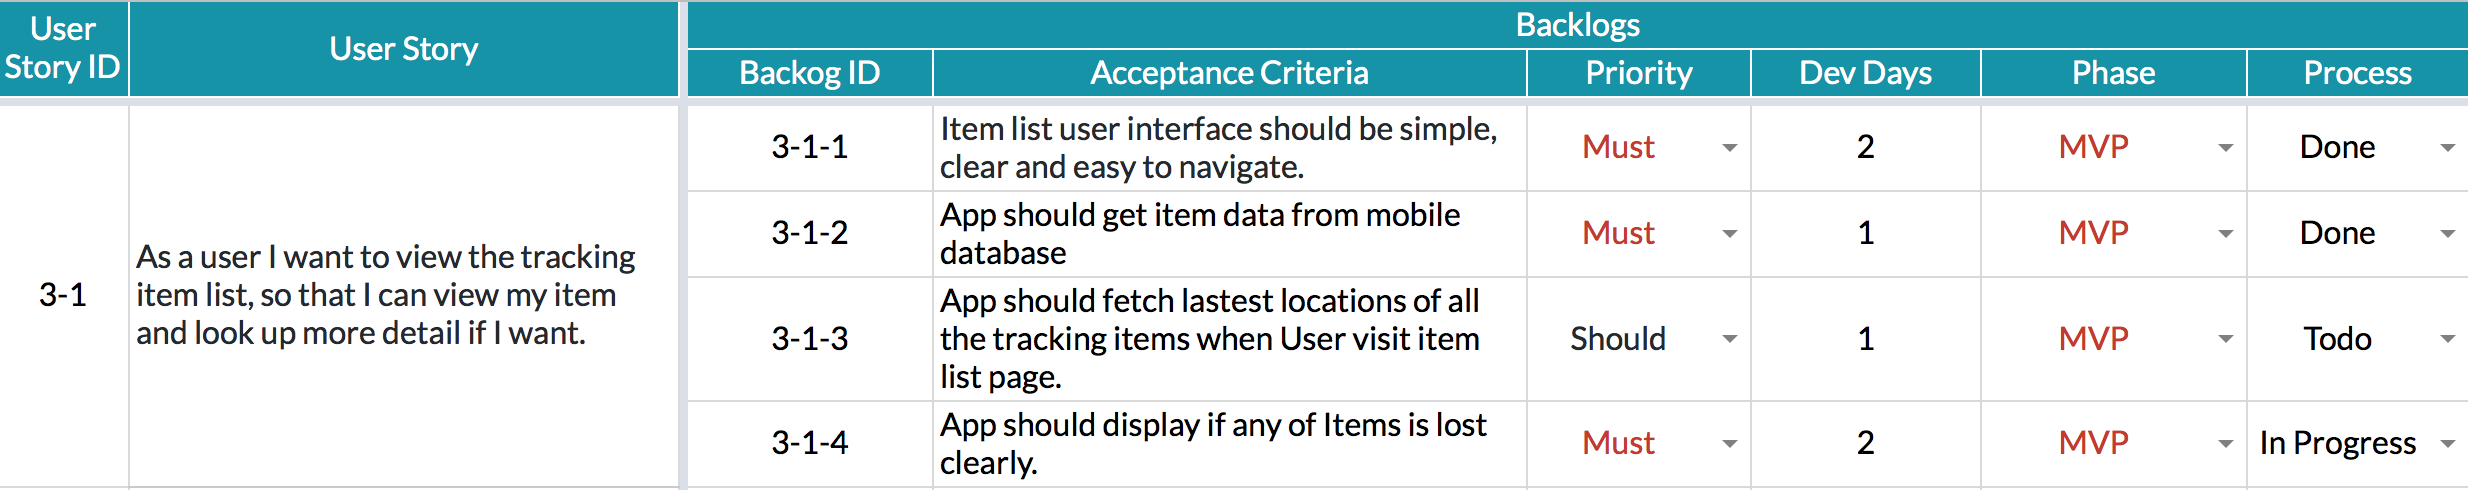
\includegraphics[width=1\textwidth]{../assets/development-records-backlog-example.png}
            \caption{Backlog Example: Sub-user story 3-1}
            \label{fig:Backlog Example: Sub-user story 3-1}
          \end{figure}
          
          The full backlogs can be found in the appendix \ref{appendix:backlogs} and it was used to create our Kanban showed in figure \ref{fig:iOS Development Kanban}, which kept the developing process recorded easily to follow.        
          
        \subsubsection{Progress Tracking}
          \paragraph{}To record our progress, we kept using the same progress tracking form as the last term, and this term we did some improvements:

          \begin{itemize}
            \item {Lock every week}: To prevent any team members from modifying the resource hours dishonestly, a range of the form was locked every week. Only records within recent two weeks were allowed to be added. 
            \item {Status documented in more detail}: To increase the traceability and convincing evidence, each resource hours commitment was asked to provide a more detailed description. Instead of {\it reporting writing}, it was improved to {\it Final report: Formative Evaluation - mobile application test}.
          \end{itemize}

          Please find the full progress tracking form in appendix \ref{appendix:progress-tracking-form}.\\
          
          Until March 16, the total working time during these two terms is {\bf 581.9 hours}. All these hours contributed includes all lab sessions, supervisor meetings, daily sprint and self-independent working time. 58.7\% was contributed by Hussein and Jheng-Hao as shown in figure \ref{fig:Progress Tracking Diagram}. The top contributor is Jheng-Hao with 222.95 hours contributed, while the last is Chin with 26.5 hours recorded. The line chart displays that the commitment became dramatically different since the start of the second term. Most of the team members stopped to work in the second term, excluding Hussein and Jheng-Hao who still kept working continuously.
          
          \begin{figure}[H]
            \centering
            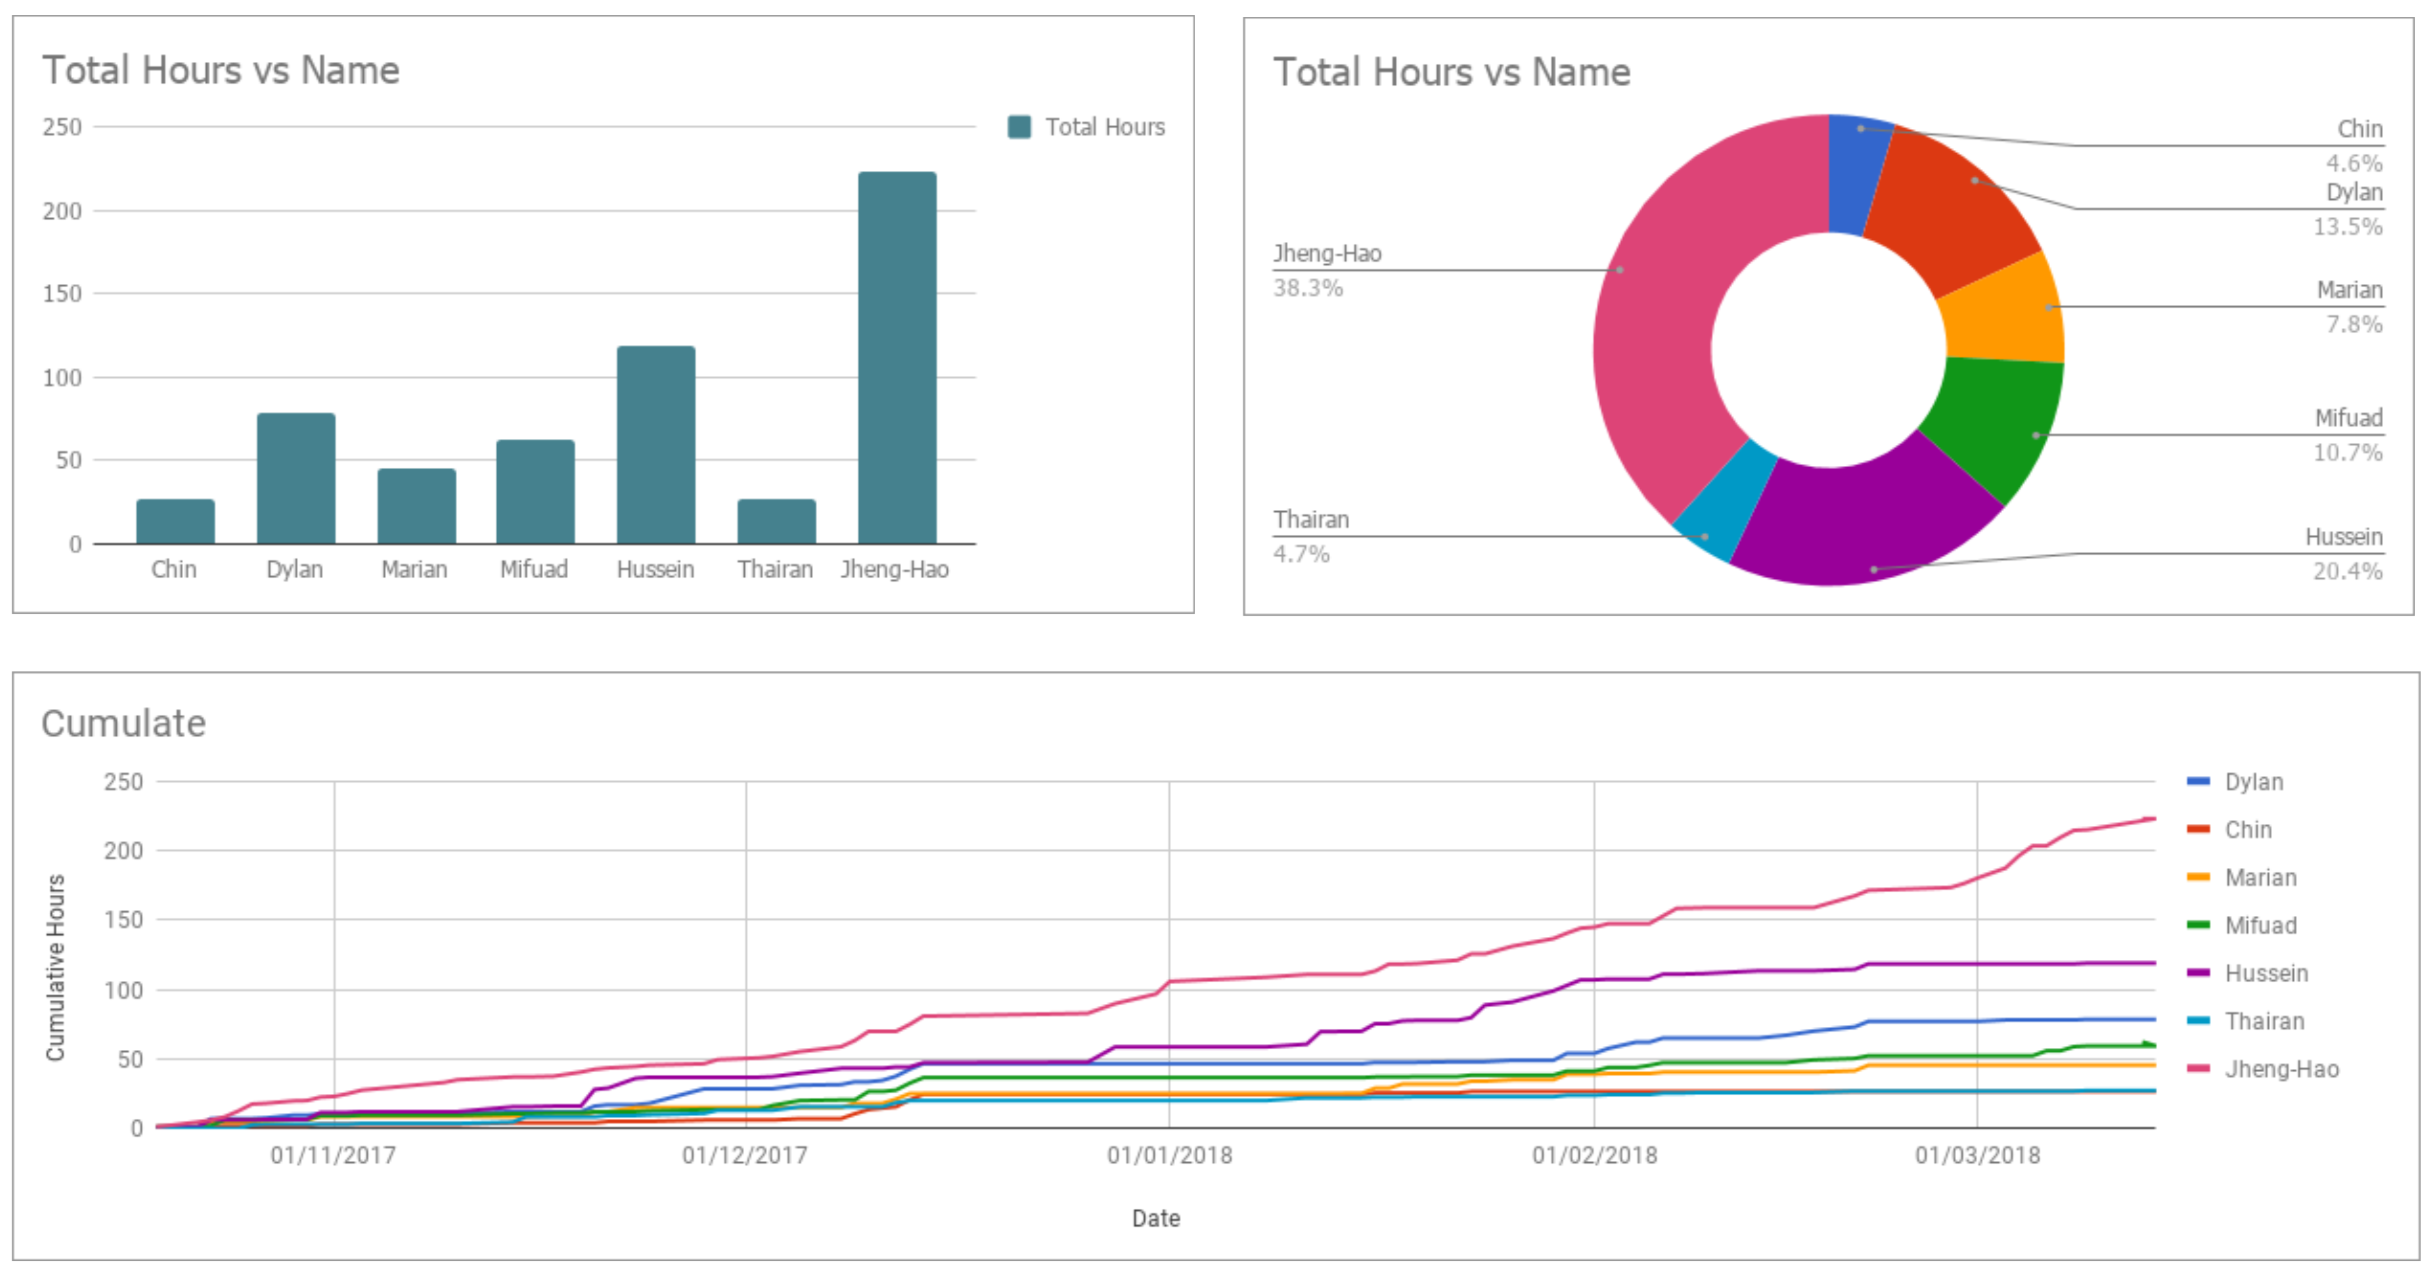
\includegraphics[width=1\textwidth]{../assets/development-records-progress-tracking-diagram.png}
            \caption{Progress Tracking Diagram (until March 16th)}
            \label{fig:Progress Tracking Diagram}
          \end{figure}

    \section{Formative Evaluation}
      \label{Chapter:Formative Evaluation}
      % total 1650 words
      \subsection{iOS App Evaluation} 
        
          % total 1000 words
        \subsubsection{Objectives and Questions}
          % 100 words
          \paragraph{}
            We wrote quantitative tasks to test the usability of our mobile application\cite{WritingTasks}. The purpose of the tests was to test if the participants can actually finish the task with the application, and we could learn from the process and observe how users used our application and improve it if any issues or confusion were raised. 

            \begin{figure}[H]
              \centering
              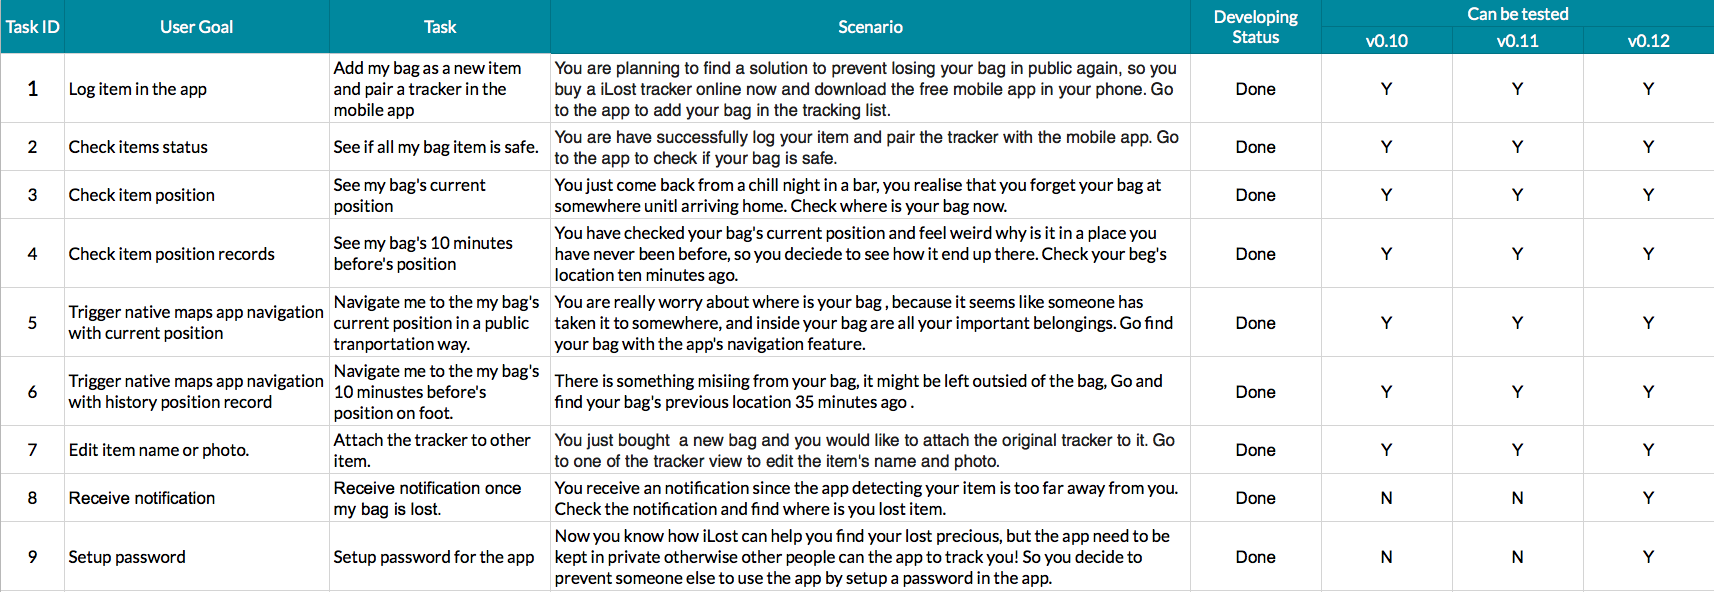
\includegraphics[width=1\textwidth]{../assets/usability-test-task-list.png}
              \caption{Usability test task list}
              \label{fig:Usability test task list}
            \end{figure}

            \begin{table}[H]
              \centering
                \begin{tabularx}{\textwidth}{l X}
                  \hline
                  Column & Description  \\ \hline
                  Task ID & Identify the number of the task.  \\ 
                  User Goal & What is the objective we need users to perform.  \\ 
                  Task & The process in terms of completing the goal.  \\ 
                  Scenario & A setup scenario for engaging testers to use the application in a real-life case.   \\ 
                  Developing Status & Current latest developing status of the functionality of this task, it should be {\bf To do}, {\bf In Progress} and {\bf Done}.\\ 
                  Can be tested &  Whether the functionality of the application is ready to be tested in each version that was created.\\ 
                  \hline
                \end{tabularx}
                \caption[Table caption text]{Usability test task list columns}
                \label{table:Usability test task list columns}
            \end{table}

            Figure \ref{fig:Usability test task list} demonstrates our tasks and goals. Table \ref{table:Usability test task list columns} shows what the columns stand for.

        \subsubsection{Participants, Location and Setup}
          % 100 words
          \paragraph{} According to Jakob Nielsen, testing 5 users in a usability study could find almost as many usability problems as testing more participants\cite{HowManyTestUsers}. Following this theory, our application was tested with 5 participants for each version that was created. The study was taken place in the library of Goldsmiths, University of London, and the participants were the students who used to bring a bag to the campus daily. In total we have conducted three versions of the application.
          
        \subsubsection{Methodology and Measures}
          % 100 words
          \paragraph{} Firstly, we explained what was our project about and asked participants to sign up the consent form which can be found in appendices \ref{appendix:consent-form}. During the test, the participants were provided an iPhone with the application built-in to test. An observer would guide them through the tasks and the scenarios, then took notes of how the participants reacted to the application. For each task, the observer would record if it was successfully completed or failed. The records would help us to build the success rate diagrams which helped us to understand which usability needed to be improved\cite{SuccessRates}. 
        
        \subsubsection{Evaluation}
          
          \begin{figure}[H]
            \centering
            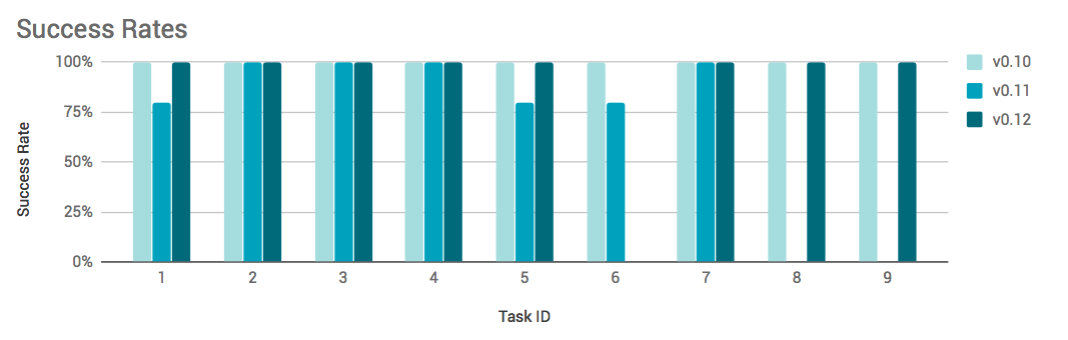
\includegraphics[width=1\textwidth]{../assets/usability-test-success-rates.png}
            \caption{iOS App Success Rates Diagram}
            \label{fig:iOS App Success Rates Diagram}
          \end{figure}

          \paragraph{v0.10} The tested subject was the application prototype built in {\bf Adobe XD}, which was one of the best design tools to test the prototype. Thanks to the well-designed user interfaces, the goals were easily achieved and the  tasks were all successful. The results only proved that the user interfaces guided the users to the right view, however it could not actually reflect on the usability of the real application. After all, Adobe XD could only let users walk through each view by clicking, while an actual iOS application would support swipe or other gestures. It was more like a paper prototype usability test.
          
          \paragraph{v0.11} We benefited most from this test since this test was the native mobile application, where the participants can actually use it like other applications. This version was built in React Native and tested in Expo which is a tool and service which we used to build the mobile native application with React Native. During this test, we received several comments towards the {\bf add item view}. For example, the camera icon in that view was originally used as a button. But some of the users could not really regard it as a button but a decoration since it was colourful. Also, the placeholder of the item name field was {\bf Item Name} instead of a prompt message which confused some of the participants as well. So after this test, we resolved the issues and the differences show in figure \ref{fig:usability-test-ios-v010-improvements}. Task 8 and 9 were not developed completely at the moment so there was not any record.

          \begin{figure}[H]
            \centering
            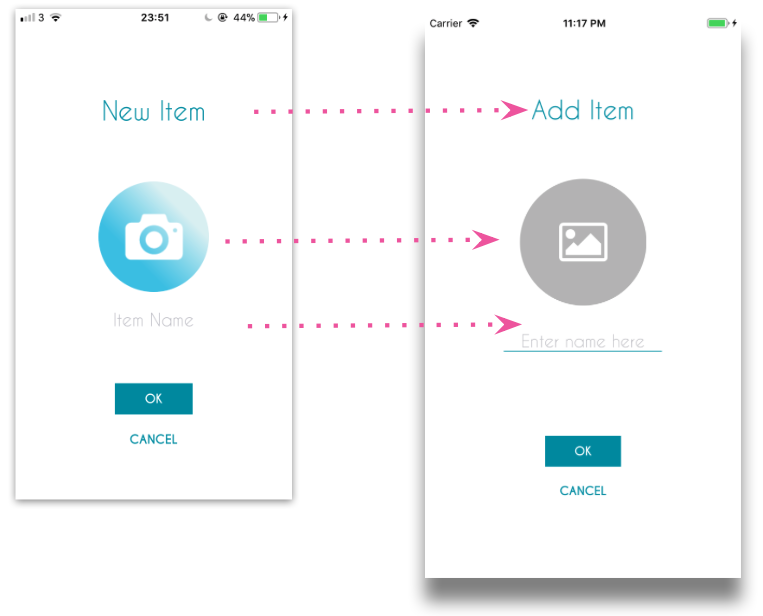
\includegraphics[width=0.7\textwidth]{../assets/usability-test-ios-v010-improvements.png}
            \caption{Improvement of the add item view}
            \label{fig:usability-test-ios-v010-improvements}
          \end{figure}

          \paragraph{v0.12} After the previous test, we not only improved some of the user interfaces but also removed some of the features. It is worth notice that there is no record of task 6, which is {\bf navigating to previous locations of the item's location history}. The reason we removed this task was that this goal was not really helpful. The participants commented that it was not beneficial to navigate to the previous locations, they cared about the current location of the item more. So thanks to the feedback, we removed task 6 and eliminated the functionality of navigating through past location history which made the application more simple. 
        
        \subsection{Conclusion}
          % 200 max words
          We found it really helpful to do the testing regularly, because what we thought the users' needs might not be true, it was quicker to hear their actual voice by conducting tests with them. In terms of the cycle of agile development, it might be really practical to conduct the tests every half month, to make sure we are on the right track and meet the users' needs.           
          Due to the time limit, we were not able to conduct the tests for the tracker unfortunately.
      
    \section{Design and Implementation}
      \subsection{Design Stage}
        \paragraph{} Our final design for the iLost tracker consists of an Android app and a Raspberry pi with the attached Hologram Nova. The User interacts with the Android app, whereas the Raspberry pi provides the short-range capability of the Bluetooth and the Hologram Nova cellular modem attached to the Raspberry pi provides the long-range capability.

        \paragraph{} Short range (figure \ref{fig:Tracker concept at January - short range}) is defined as less than 30 metres from the target and long-range (figure \ref{fig:Tracker concept at January - long range}) is defined as above 30 metres to 400 km and beyond.
        
        \begin{figure}[H]
          \centering
          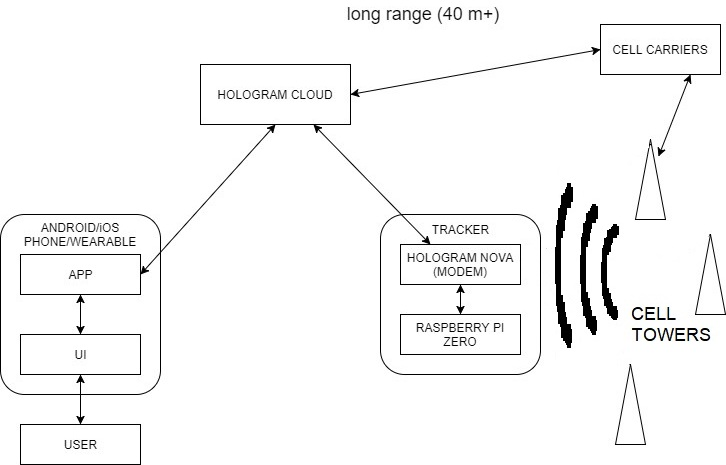
\includegraphics[width=0.8\textwidth]{../assets/design-concept-v20-long-range.jpg}
          \caption{Tracker concept 2.0 at January - long range}
          \label{fig:Tracker concept at January - long range}
        \end{figure}
        
        \begin{figure}[H]
          \centering
          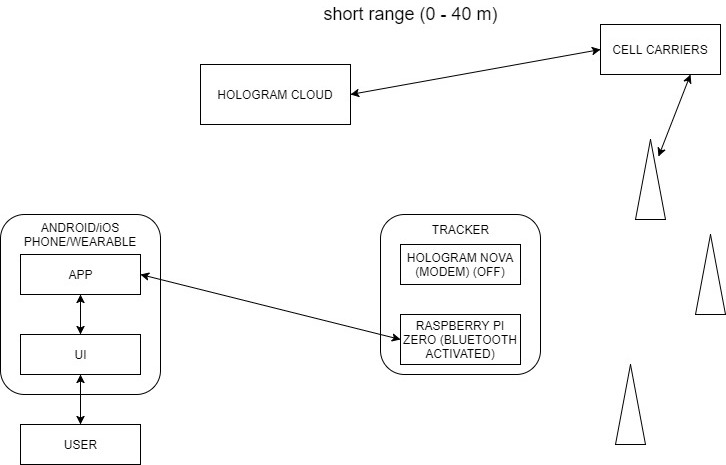
\includegraphics[width=0.8\textwidth]{../assets/design-concept-v20-short-range.jpg}
          \caption{Tracker concept 2.0 at January - short range}
          \label{fig:Tracker concept at January - short range}
        \end{figure}
        
        \paragraph{} This Hybrid approach, compensates for the weaknesses of the Bluetooth range and the weaknesses of the accuracy of the Hologram Cellular modem, by leveraging the short-range accuracy of the Bluetooth and extremely long range of the cellular modem. (There are cell towers in nearly every part of the world.)
        
        \paragraph{} In our final design, considering the strong demand from users to have the tracker as small as possible (similar to the Tile Mate in figure \ref{fig:Tile Mate}). We endeavoured to ensure the tracker is compact as possible.
        
        \paragraph{} We also initially designed the Tracker to be server-less. In this way, the tracker would communicate and share information directly with the users iLost app.
        
        \paragraph{} Moreover, we set out to have the tracker adapt to the users need. The iLost tracker should be able to be smart enough to understand that a user has left behind an item regardless of the item type (luggage, handbag, laptop etc.) However, our design plan changed rapidly as we started implementing the tracker and as we consulted with more users and professionals (both in marketing and in engineering).
        
        \begin{figure}[H]
          \centering
          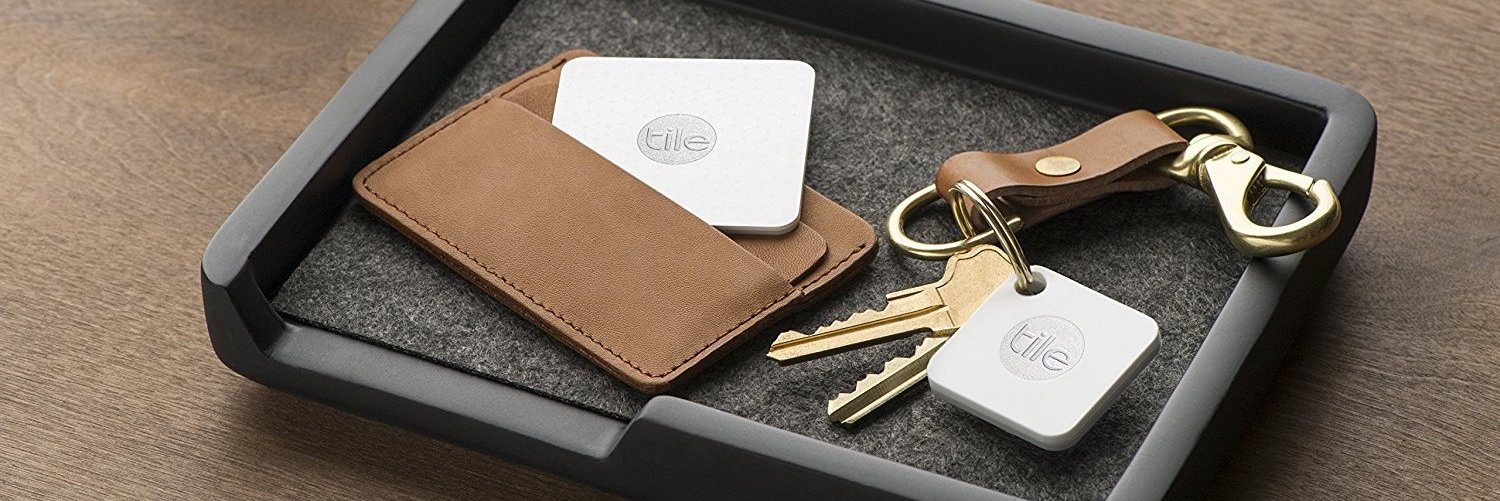
\includegraphics[width=0.7\textwidth]{../assets/design-concept-tile-mate.jpg}
          \caption{Tile Mate}
          \label{fig:Tile Mate}
        \end{figure}
        
        \paragraph{} At the computer fair, in which we consulted with various industry professionals, we realised that we should focus on a minimum viable product for the duration of this project. Certain product features such as having the tracker as physically small as a sticker (similar to the Tile Mate) is not possible in the scope of the project as we need specialist manufacturers, engineers and funding (we already looked at all the possible routes to making the tracker smaller). Most users clearly want a tracker that is as small as Tile Mate, so we looked at the next viable use case and the minimum physical size of the tracker that can fit that viable use case, this was baggage use case. 

        \paragraph{} The posters for the computer fair can be found in appendix \ref{appendix:computer-fair-posters}. 
        
        \paragraph{} It is feasible in the time frame and available resources in this project, to build a physical tracker that is small enough (insert dimensions here) to fit in the user’s handbag, rucksack and travel luggage (the baggage use case). While also available to fulfil the user criteria in terms of accurate, long range tracking (over 30 metres).
        
        \paragraph{} At the design stage, we initially designed the tracker to be server-less i.e. The physical tracker solely communicates via cellular data to the app on the users phone, reducing cost and increasing security for the user. However, for the cellular modem to function properly, it must communicate with the Hologram Nova cloud servers, this is so that the Hologram can negotiate with multiple phone carriers, this functionality allows the user with one sim card to able to have a tracker that can triangulate and transmit data anywhere in the world which has cell towers.
        
        \paragraph{} Currently the tracker communicates with the Hologram Cloud servers, which in turn communicates with the user’s app.
        
        \paragraph{} Also, in the design stage we realised that our tracker can be developed into an enterprise framework. If our product is successful at item tracking for consumers and is fully tried and tested, this same technology can be used for enterprise applications, such as asset tracking, shipment tracking, even livestock tracking. However, this is not in the scope of this project.
        
      \subsection{Implementation Stage}

        \paragraph{} We initially designed the user app to be hosted on the Android platform, instead we implemented the user app on both the iOS and the Android platform. We did this for two reasons. Firstly, from market research shown in figure \ref{fig:Mobile OS Market Research in UK}, roughly 53\% of users do not have an Android smartphone. Secondly, developing the Android app allows us to have a plan B, in case we cannot develop the iOS app in time or if there are compatibility issues with the tracker. The Android and iOS app both have different programming languages and paradigms. 

        \begin{figure}[H]
          \centering
          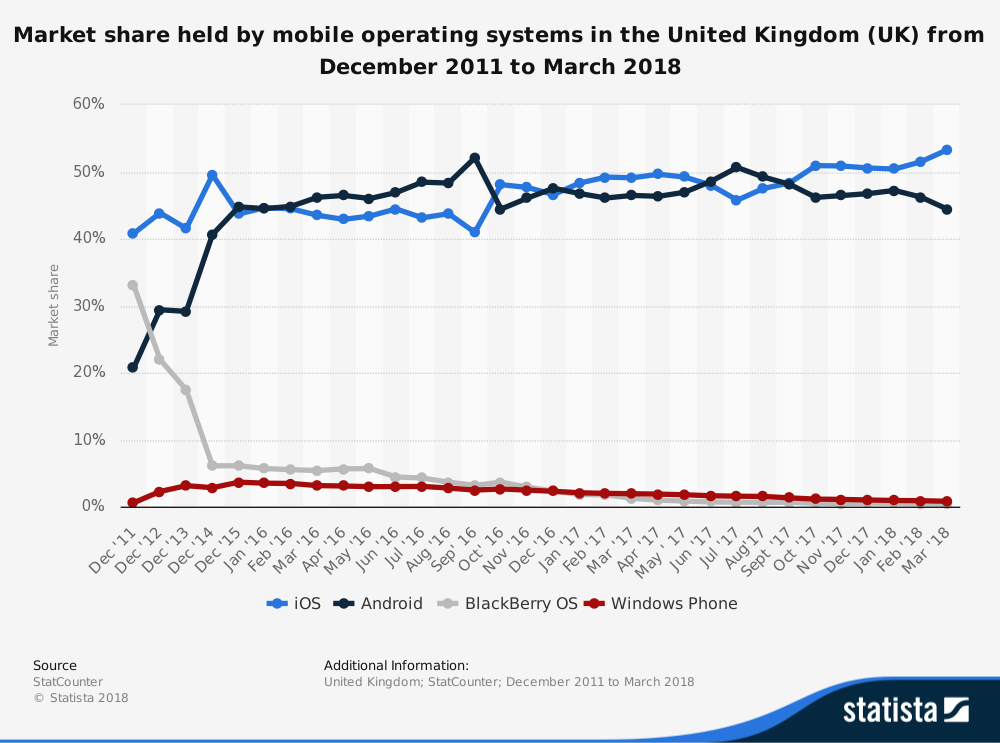
\includegraphics[width=0.7\textwidth]{../assets/design-implement-stage-market-research.png}
          \caption{Mobile OS Market Reseatch in UK \cite{MobileOSMarketShare}}
          \label{fig:Mobile OS Market Reseatch in UK}
        \end{figure}
        
        \paragraph{} The reason why we developed an Android/iOS app instead of a web app, is that as part of the iLost design, the user needs notifications in real-time (when an item has been left behind). Real-time notifications are not currently possible with web apps.
        
        \paragraph{} Another significant change to the iLost tracker was the discarding of the Bluetooth function. Initially, the iLost tracker was supposed to use the Generic Bluetooth adapter on the Raspberry pi and the user’s smartphone.  
        
        \paragraph{} The Bluetooth function is needed for the tracker at short range (less than 30 metres) to remind the user if they have left an item behind, if an individual recently just stole their item or for tracking down the location of an item (to a range +- 5 metres). This is after the long-range function (i.e. the cellular modem) locates a rough location of the item (30-40 metres from actual location)
        
        \paragraph{} In a situation whereby, the user is greater than 30 metres away from the physical tracker but requires a more precise location of the tracker, the Bluetooth function was supposed to fulfil this use case. My measuring Bluetooth signal strength coming out of the tracker, (2.4 to 2.485 GHz radio frequencies) the user can determine how near they are to the tracker and thereby their lost/stolen item. 
        
        \paragraph{} However, although the Bluetooth concept is simple, as many developers (we talked with one personally in the department) implementing reliable Bluetooth functionality is problematic (looking at most Bluetooth products on the market, many products have connectivity problems).  
        
        \paragraph{} The main disadvantage that led us to cancelling the Bluetooth function, is that in order to support the iOS platform for the users, the iLost tracker must comply with MFi (Made For iPhone) program. The MFi program restricts the types of devices that can connect to Apple products. The iLost tracker is a Raspberry pi with an attached cellular modem, the Raspberry pi is not certified under the MFi program. This means the iLost tracker Bluetooth function (it’s a Raspberry pi zero, which has a Bluetooth module by default) cannot interact with the user app and we cannot release the iLost tracker for the iOS platform.
        
        \paragraph{} Subsequently, we tried to implement the iLost Bluetooth feature with the Android app. Although, the Android platform did not have a compliance program like the iOS, there were other serious issues. We simply could not find the functionality to be able to measure the Bluetooth signal strength emitting from the iLost tracker.  We assumed that the mac address of the iLost tracker would always be the same, but this is not correct. After Bluetooth 4.2 was released, the mac addresses of any Bluetooth device is constantly randomised. Because the mac addresses (we need this address to communicate with the iLost tracker) is randomised we cannot from Android app side be certain which Bluetooth device is the iLost tracker. 
        
        \paragraph{} We also looked at other Bluetooth products on the market, such as most headphones. They were also plagued with stability issues (such as signal not receiving or pairing breaking), if we were to implement the Bluetooth feature we would need experienced developers who specialise in implementing reliable Bluetooth communications between user apps and physical computing devices. Unfortunately, there is also no library or service (like Hologram) which simplifies the Bluetooth stack. 
        
        \paragraph{} Moreover, we experimented with other Bluetooth based technologies, to find a replacement. We tested and built mock-ups using the estimote beacon (a Bluetooth tracker, used in upcoming retail and asset tracking), this did not fit our use case, as it increased unnecessary cost and complications to the user. Another novel Bluetooth tracker which failed the use case was the puck.js (a small Bluetooth tracker that can programmed using JavaScript) although a novel concept, we did not possess enough technical skill to be able to program the Puck to detect it to read Bluetooth signals specifically emitting from the raspberry Pi. 
        
        % [insert picture of Raspberry pi 3 model B with hologram nova attached, we need to take a picture of this]
        
        \paragraph{} Our next step, was to implement the Cellular functionality of the iLost tracker. The cellular functionality consists of a cellular modem (called Hologram Nova) provided by the company Hologram. The Hologram Nova, via USB is attached to the Raspberry pi (for testing and early prototyping we used the Raspberry pi 3 model B) and this is what we refer to as the iLost tracker. We managed to establish a protocol to communicate with the iLost tracker.
        
        \paragraph{} This protocol consists of sending HTTP requests to the tracker, the tracker then responds via HTTP post with the data back to the sender.   
        
        \paragraph{} At first, we sent HTTP requests via our computers (using the Postman application) to the iLost tracker, we received responses that showed that the communication method functioned. 
        
        \paragraph{} After, we checked that the cellular modem method of location worked and that it could return useful data. The Hologram Nova uses nearby cell towers to triangulate its location. It did work, but the accuracy was not satisfactory, on average location was 40 metres away from the bag we were tracking.
        
        \paragraph{} Even though we could send HTTP requests to the tracker as well as sending simple worded messages (such as “RL” for request location), we could not request the tracker to send its location back to the sender.
        
        \paragraph{} So, we needed to solve this issue. At first, we tried to set up an apache web server on the Raspberry pi, open a specified port on the server and send messages to that port. We built a python script that would reply to any specified message we sent to the server. This did not work, any messages we sent were not received by the server. What we didn’t realise was that when we were sending a message to the tracker, the payload was being sent to the Hologram Cloud servers, these cloud servers would then forward the payload directly to the tracker.
        
        \paragraph{} We could not find a way around the Hologram cloud servers, in fact the Hologram cloud servers were essential. They reason why their cloud servers are needed is that in order for us to communicate with the Hologram nova (cellular modem) and be able to triangulate the location of the tracker (i.e. Raspberry pi), the Hologram service as a whole needs to negotiate with multiple mobile network carriers. Being able to triangulate location using cell towers and communicate with a cellular modem internationally at a regular price (it currently costs us \$1 a month) is only possible currently using the Hologram service. Previously developers had overcome many administrative, legal and economic issue in order to work with cellular networks.  
        
        \paragraph{} Through all our testing and use the Cloud servers did not fail and reliably delivered any payloads we sent to the tracker. Without the Apache server, we then used Hologram SDK (which includes a Command Line interface) to open a server at port 4010 (on the Raspberry pi), any messages we sent via HTTP were now received (we could view the message on a terminal) we then used Bash scripts to automate useful responses. For example, if the message “RL” was sent (Request Location) then the tracker via the scripts would triangulate its location, store this data (longitude, latitude, altitude) as string data and send this back to the sender. Scripts were also created for the tracker to shut itself down, power itself up, disconnect from cellular networks (use cases such as the user traveling on an airline).
        
        \paragraph{} We also tried to host a server on Igor instead of the Raspberry pi, however we found a more efficient solution, this was to leverage the Hologram Cloud servers. The Igor servers are not available worldwide and offered limited scalability. 
        
        \paragraph{} The reason why Bash scripts were used instead of python is that there is native support for using CLI commands provided by the Hologram SDK. Another advantage of using Bash scripts were that we were able turn these scripts into daemons. Daemons are process that run without user supervision and in the background on Unix/Unix-like operating systems. The cron (specifically crontab) program is used and whenever the tracker is turned on, all of the Bash scripts that enable tracker functionality run as background processes, lowering the power consumption of the tracker.
        
        \paragraph{} Using a Bash script, and using inbuilt Linux programs such as grep, cron, is in line with the Unix philosophy of small programs which do one specific function efficiently, being chained together to build a larger program. 
        
        \paragraph{} Even though we could request the tracker to send its location back successfully, we still needed to be able to store this data, so the user app could access it and use it. We researched into the possibility of running a small server on the user app, which could receive this data. This is not possible; Any server must operate outside of iOS and Android platform.
        
        \paragraph{} We then decided to use the Amazon s3 servers which are scalable (servers can be replicated or moved to any AWS region), reliable (good track record, enterprise grade), available worldwide and inexpensive. The tracker now sends location data to our s3 server. We were then able to have the user app request location data from the s3 server and display this data/their location of the tracker to the user.
        
        \paragraph{} We also encrypted this data using AES-256 servers side encryption keys, each record is encrypted with a unique key, even the key itself is regularly encrypted. This service is provided by Amazon.
        
        \begin{figure}[H]
          \centering
          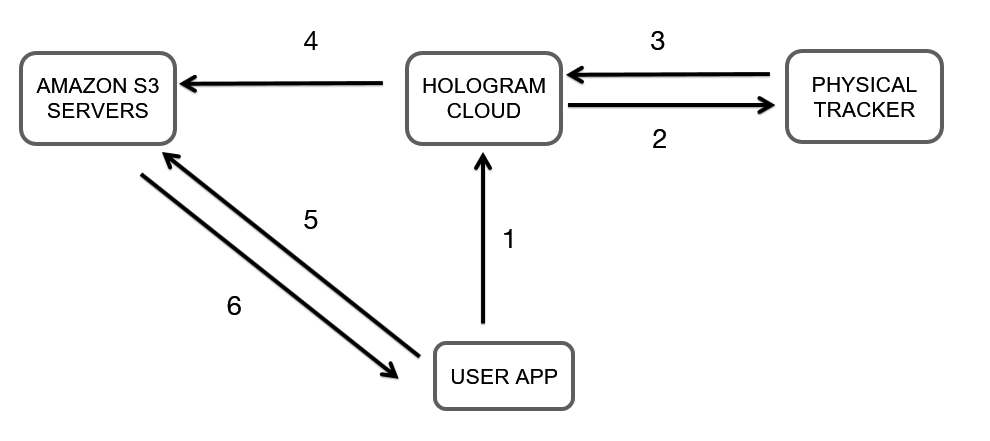
\includegraphics[width=0.7\textwidth]{../assets/design-implement-stage-current-stack.png}
          \caption{Current Stack}
          \label{fig:Current Stack}
        \end{figure}

        \paragraph{} Post-Snowden age, we understand users are concerned about privacy. All data that is stored on Amazon servers are automatically encrypted by AES-256 servers side encryption keys. We only store longitude, latitude and time data, for 14 days. It saves us space and cost, to not store data permanently.
        
        \paragraph{} Location data such as longitude and latitude is metadata, its ambiguous not content that can identify the users personal information. The purpose of the Amazon server is only required to provide data back to the user. Also, each tracker has an unique ID number, personal information is not identifiable from this data. 
        
        \paragraph{} We cannot guarantee compliance with UK Data protection act, due to the legal complexity of having the Amazon operating servers globally as well as the Hologram Nova having to operate with many network carriers globally. Ideally, with more funding we would be able to consult with legal professionals. 
        
        \paragraph{} Next, we needed to create the UI for the iOS app and Android app. We approached this by keeping everything as minimal and simple as possible for the user. The user would take a picture of the item they want to track and assign a category for it. When the user wants the location of their bag for example they would tap on the “[locate]” button, a Google map view of their item would show along with any information such as directions and distance. 
        
        \paragraph{} However, we migrated from the iOS app being built in the swift language to React Native. React Native is a framework that allows developers to build mobile apps for both the iOS and Android platform using JavaScript and the React framework. 
        
        \paragraph{} At the beginning of the project, our iOS developer team did not have experience with using the Swift language and associated frameworks. We spent 3 - 4 weeks building a basic application which only had a tab bar view to switch between pages, and only half of the user interface components were functional. 

        \paragraph{} The Android app and iOS app user interface design can be found in figure \ref{fig:Android App User interface Design} and figure \ref{fig:iOS App User interface Design}.
        
        \paragraph{} Due to the limited development time, we searched for an alternative method that would reduce development time. We found that React Native and Flutter were good alternatives to develop native mobile applications. React Native was chosen because it was more mature than Flutter, which was relatively unstable as it had just been released. Unexpectedly, only three days were required to develop the same application, which the iOS team spent almost a month to build, in React Native. Switching to React Native was a good decision as it significantly shortened the development time providing us more time to do usability tests.
        
        \paragraph{} The iOS team also had previous experience in developing React web applications, where React shares the same component-based concept and reactive function programming paradigm with React Native. Also, React Native uses JavaScript which we were more familiar with, so it was relatively easier for us to develop the application.
        
        \paragraph{} The Swift API had many noteworthy changes from Swift 2.0 to 4.0 which is the latest version (we were developing with latest version), so whenever we encountered an issue, it was difficult to search for the solution for the latest version of Swift. The official documentation of Swift was also quite ambiguous, it lacked working examples. This led to a steep of learning curve when developing in Swift. On the other hand, React Native had better documentations and community support. The official documentation was explained clearly with good working examples, there were more community-built components that can be approached easily as well, this improved the developing experience and made it easier.
        
        \begin{figure}[H]
          \centering
          \begin{tabular}{ccccc}
            \subfloat[Welcome-1]{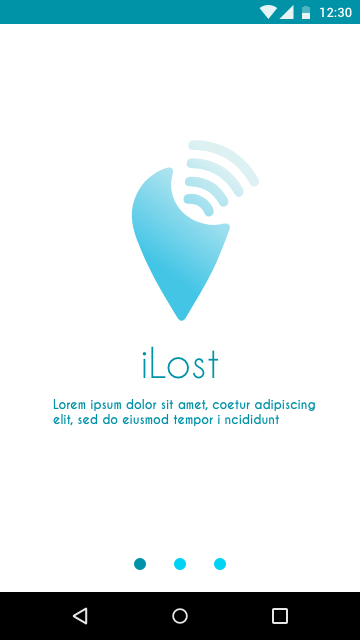
\includegraphics[width = 1.5in]{../assets/android-ui/1-1-welcome-1.jpg}} &
            \subfloat[Welcome-2]{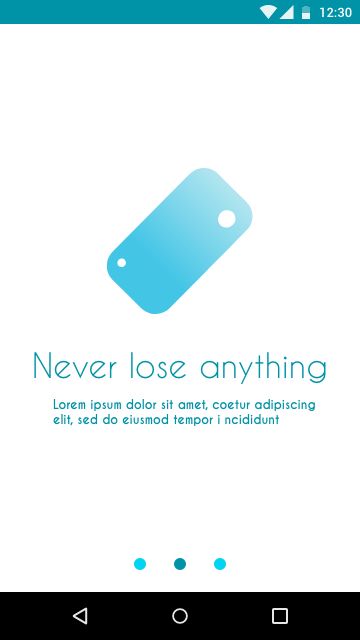
\includegraphics[width = 1.5in]{../assets/android-ui/1-2-welcome-2.jpg}} &
            \subfloat[Welcome-3]{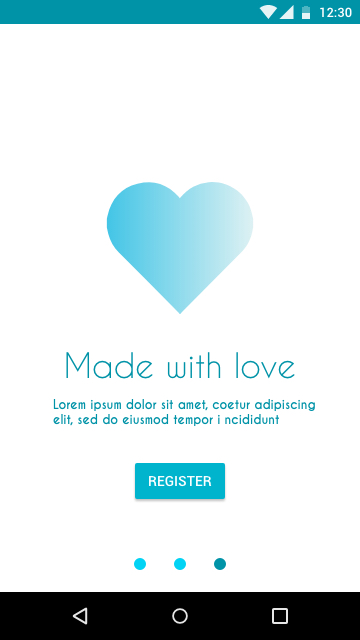
\includegraphics[width = 1.5in]{../assets/android-ui/1-3-welcome-3.jpg}} &
            \subfloat[Register]{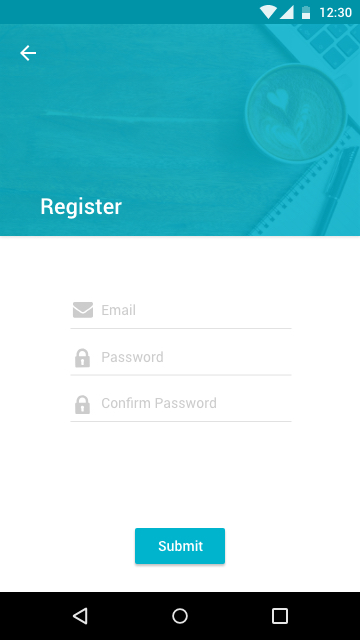
\includegraphics[width = 1.5in]{../assets/android-ui/2-1-register.jpg}} \\
            \subfloat[Register Succeed]{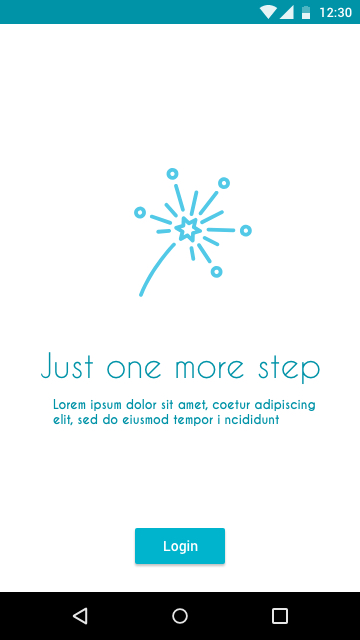
\includegraphics[width = 1.5in]{../assets/android-ui/2-2-register-succeed.jpg}} &
            \subfloat[Login]{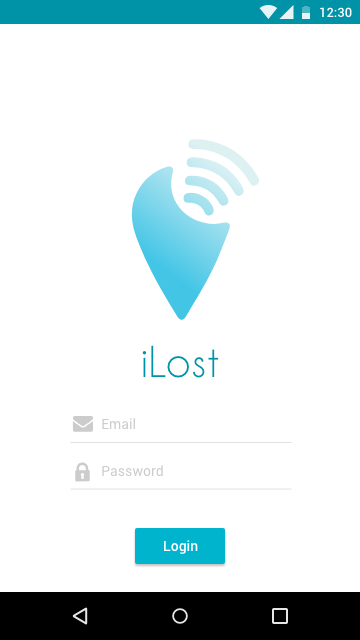
\includegraphics[width = 1.5in]{../assets/android-ui/2-3-login.jpg}} &
            \subfloat[Item List]{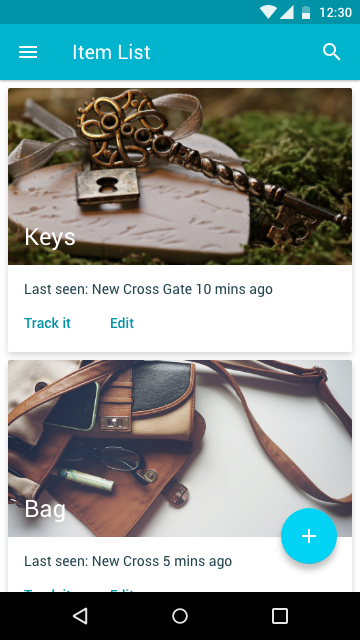
\includegraphics[width = 1.5in]{../assets/android-ui/4-1-item-list.jpg}} &
            \subfloat[Track Item]{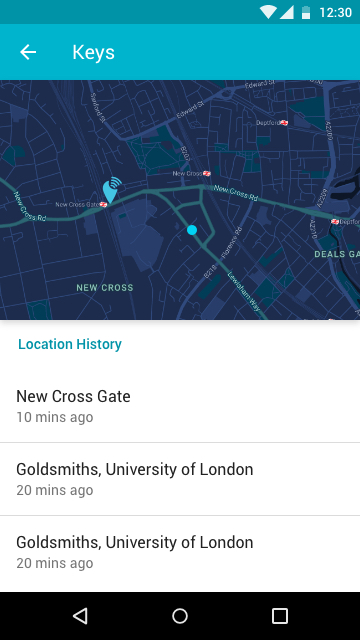
\includegraphics[width = 1.5in]{../assets/android-ui/4-2-track-item.jpg}} \\
            \subfloat[Menu]{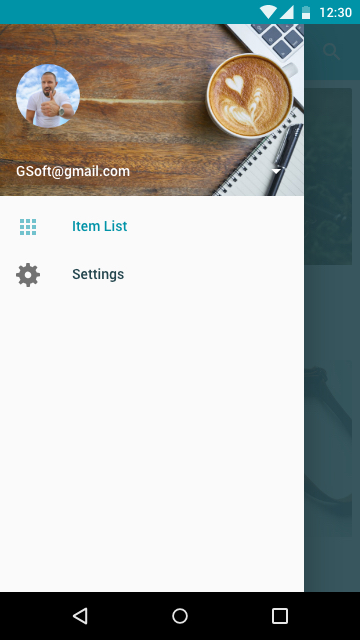
\includegraphics[width = 1.5in]{../assets/android-ui/4-3-menu.jpg}} &
            \subfloat[Add Item Photo]{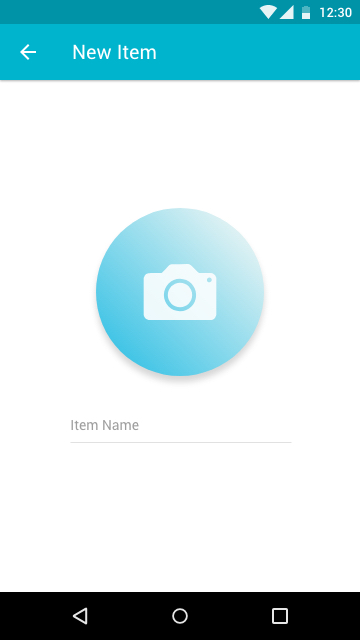
\includegraphics[width = 1.5in]{../assets/android-ui/5-1-add-a-new-item-1-photo.jpg}} &
            \subfloat[Add Item Name]{\includegraphics[width = 1.5in]{../assets/android-ui/5-2-add-a-new-item–2-name.jpg}} \\          
          \end{tabular}
        \end{figure}

        \begin{figure}[H]
          \centering
          \begin{tabular}{ccccc}
            \subfloat[Pair Tracker]{\includegraphics[width = 1.5in]{../assets/android-ui/5-3-add-a-new-item–3-pair-tracker.jpg}} &
            \subfloat[Pair Tracker Succeed]{\includegraphics[width = 1.5in]{../assets/android-ui/5-4-add-a-new-item–4-pair-tracker-succeed.jpg}} &
            \subfloat[Pair Tracker Fail]{\includegraphics[width = 1.5in]{../assets/android-ui/5-5-add-a-new-item–5-pair-tracker-fail.jpg}} &
            \subfloat[Settings]{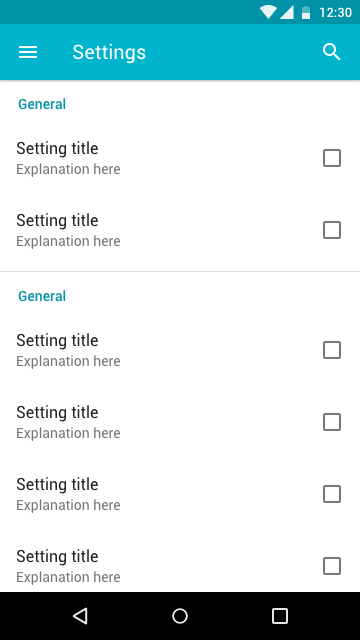
\includegraphics[width = 1.5in]{../assets/android-ui/6-1-settings.jpg}} \\
            \subfloat[Setting Menu]{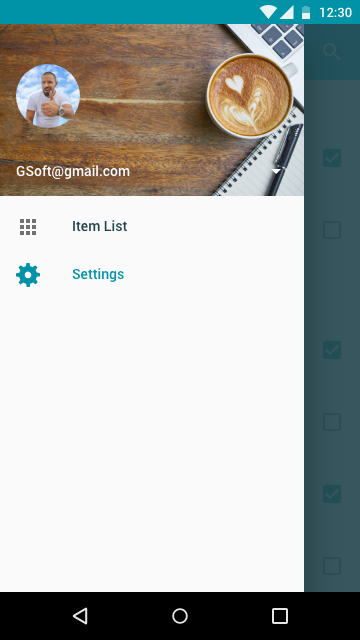
\includegraphics[width = 1.5in]{../assets/android-ui/6-2-settings-menu.jpg}}\\
          \end{tabular}
          \caption{Android App User interface Design}\label{fig:Android App User interface Design}
        \end{figure}

        \begin{figure}[H]
          \centering
          \begin{tabular}{ccccc}
            \subfloat[Welcome-1]{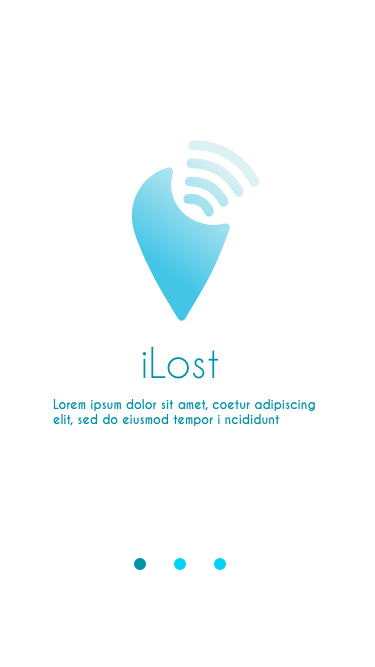
\includegraphics[width = 1.3in]{../assets/ios-ui/1-1-welcome-1.jpg}} &
            \subfloat[Welcome-2]{\includegraphics[width = 1.3in]{../assets/ios-ui/1-2-welcome–2.jpg}} &
            \subfloat[Welcome-3]{\includegraphics[width = 1.3in]{../assets/ios-ui/1-3-welcome–3.jpg}} &
            \subfloat[Register]{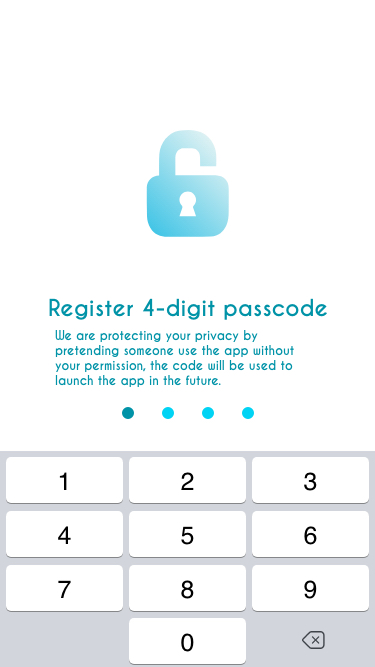
\includegraphics[width = 1.3in]{../assets/ios-ui/2-1-register.jpg}} \\
            \subfloat[Register Passcode]{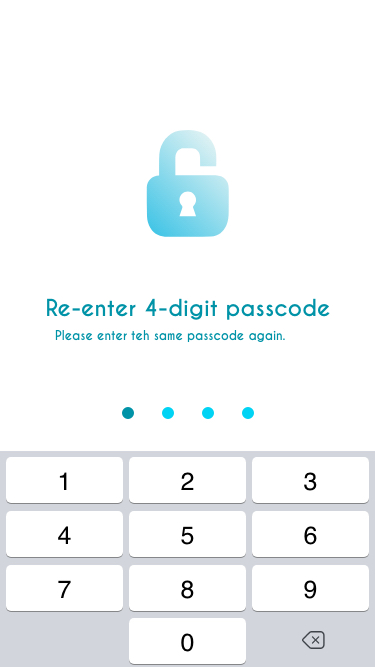
\includegraphics[width = 1.3in]{../assets/ios-ui/2-2-register-passcode.jpg}} &
            \subfloat[Register Touch ID]{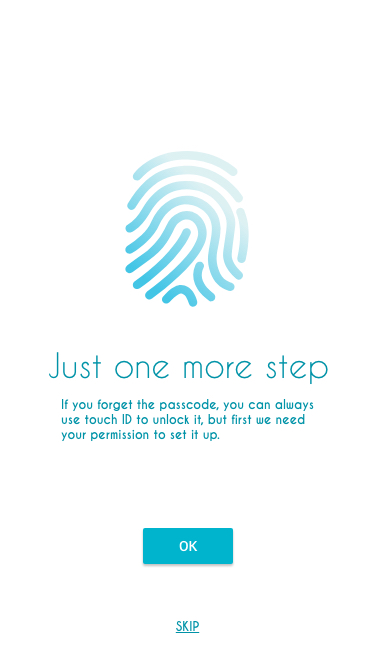
\includegraphics[width = 1.3in]{../assets/ios-ui/2-3-register-touch-ID.jpg}} &
            \subfloat[Register Touch ID Succeed]{\includegraphics[width = 1.3in]{../assets/ios-ui/2-4-register-touch-ID–success.jpg}} &
            \subfloat[Login]{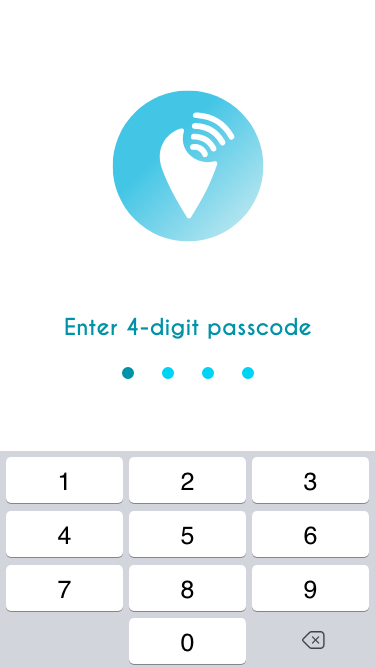
\includegraphics[width = 1.3in]{../assets/ios-ui/3-1-login.jpg}} \\
            \subfloat[Item List]{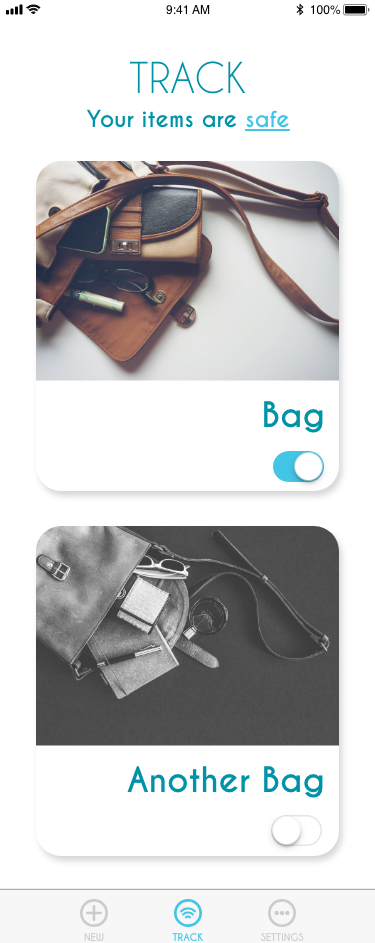
\includegraphics[width = 1.3in]{../assets/ios-ui/4-1-item-list}} & 
            \subfloat[Add a new Item - Track Item]{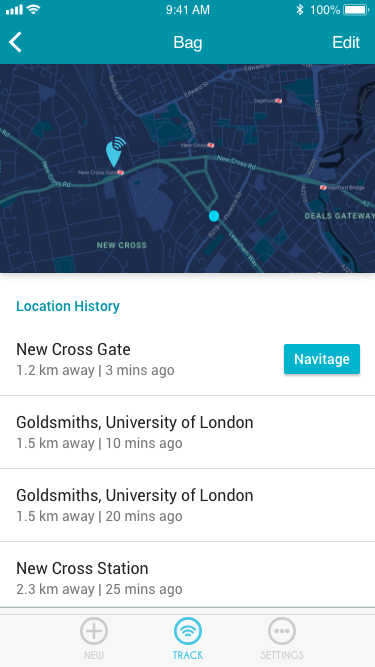
\includegraphics[width = 1.5in]{../assets/ios-ui/4-2-track-item.jpg}} &
            \subfloat[Add a new Item - Edit Item]{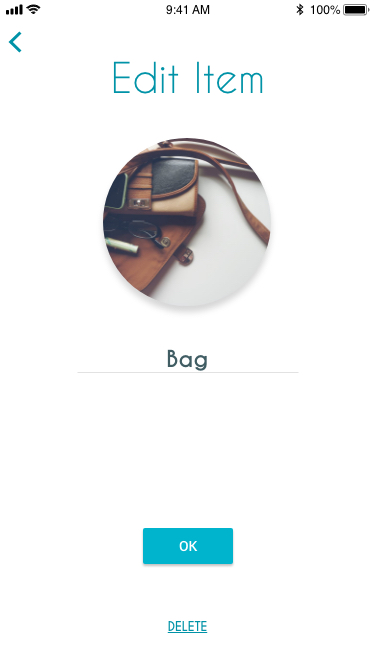
\includegraphics[width = 1.5in]{../assets/ios-ui/4-3-edit-item.jpg}} &
            \subfloat[Add a new Item - Photo]{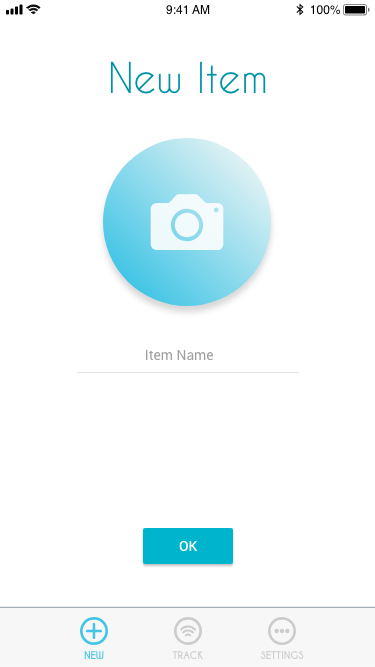
\includegraphics[width = 1.5in]{../assets/ios-ui/5-1-add-a-new-item-1-photo.jpg}}\\
          \end{tabular}
        \end{figure}

        \begin{figure}[H]
          \centering
          \begin{tabular}{ccccc}
            \subfloat[Add a new Item - Name]{\includegraphics[width = 1.5in]{../assets/ios-ui/5-2-add-a-new-item–2-name.jpg}} &
            \subfloat[Add a new Item - Pair Tracker ]{\includegraphics[width = 1.5in]{../assets/ios-ui/5-3-add-a-new-item–3-pair-tracker.jpg}} &
            \subfloat[Add a new Item - Pair Tracker Succeed]{\includegraphics[width = 1.5in]{../assets/ios-ui/5-4-add-a-new-item–4-pair-tracker-succeed.jpg}} &
            \subfloat[Add a new Item - Pair Tracker Fail]{\includegraphics[width = 1.5in]{../assets/ios-ui/5-5-add-a-new-item–5-pair-tracker-fail.jpg}} \\
            \subfloat[Setting Menu]{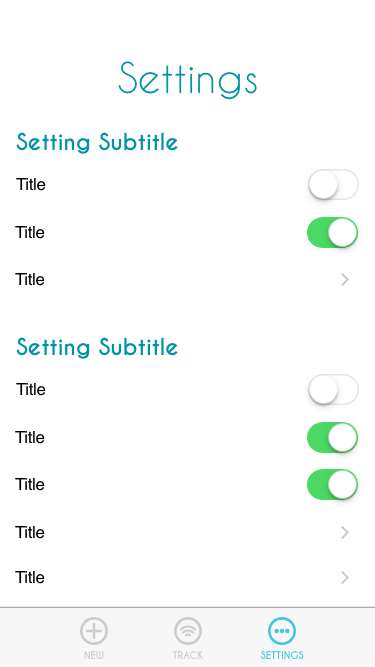
\includegraphics[width = 1.5in]{../assets/ios-ui/6-1-settings.jpg}}\\
          \end{tabular}
          \caption{iOS App User interface Design}\label{fig:iOS App User interface Design}
        \end{figure}
        
        \paragraph{} For our tracker to be useful and satisfy its use cases it had to be portable. When we were testing our tracker, which was a Raspberry pi 3 model b, it had to be plugged into the mains. We replaced the Raspberry pi 3 model b with the Raspberry pi zero. The Raspberry pi zero is 2x smaller than the Raspberry pi 3 and uses much less power and still uses the same operating system (so all the Bash scripts and configurations still worked).
        
        \paragraph{} We first tried to use small power banks to power the tracker (normally used for mobile phones) to test the average power consumption of the tracker. The tracker requires 130 mA. Using power banks is not practical for the user, so instead we tested lithium-ion batteries, these were slim and provided more power. 
        
        % We used 1200 mAH batteries, current testing shows that the tracker can last....
        % Note: I deleted this line because it's not finished yet.
        
        % \paragraph{} We have a method of charging the battery, but this requires us to remove the power cable connecting the battery to the Raspberry pi zero, there is at the moment no option for the user to charge the device...  
        % [not finished yet] 
      
        \begin{figure}[H]
          \centering
          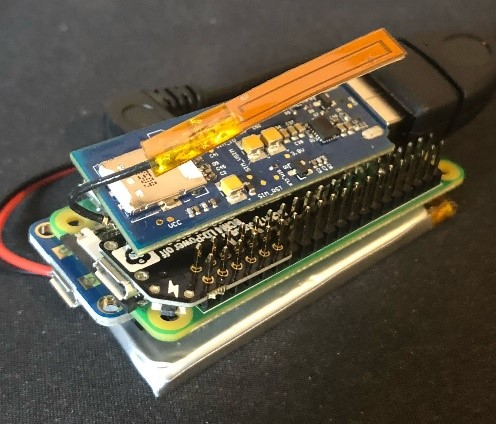
\includegraphics[width=0.7\textwidth]{../assets/design-tracker-without-case.jpg}
          \caption{Tracker without case}
          \label{fig:Tracker without case}
        \end{figure}

        \begin{figure}[H]
          \centering
          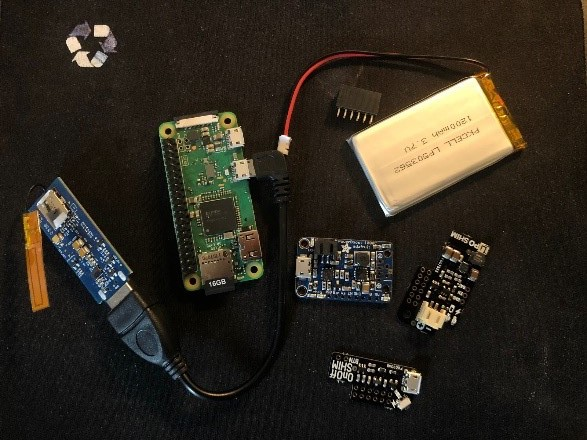
\includegraphics[width=0.7\textwidth]{../assets/design-tracker-with-all-components.jpg}
          \caption{Tracker with all components}
          \label{fig:Tracker with all components}
        \end{figure}
        
        \paragraph{} Moreover, a physical case which would fulfil the user use cases was needed for the tracker. Namely, it needed to be reasonably drop proof, strong enough to withstand day to day life, durable, simple and functional enough to be attached to a bag or another belonging. A prototype was created using laser-cut cardboard, which was interlocking. As a first iteration, it was useful as it allowed us to show to the users how our Physical tracker would look, in terms of size (how it compared to other items an user may carry), this iteration was also low cost as it was made from cardboard. By creating the first iteration, we could also see dimensions required for the internal components of the tracker and how these components would behave inside an enclosed space.
        
        \paragraph{} Some members of team also undertook 3D printing training, the 3D model design shows in figure \ref{fig:Concept Tracker Case 1} and figure \ref{fig:Concept Tracker Case 2}. Ideally, we wanted the case to be 3D printed, unfortunately we did not have enough time to progress beyond the cardboard prototype, which shows in figure \ref{fig:Concept Tracker Demo}.
        
        \begin{figure}[H]
          \centering
          \includegraphics[width=0.7\textwidth]{../assets/design-tracker-case-design-1.jpg}
          \caption{Concept Tracker Case 1}
          \label{fig:Concept Tracker Case 1}
        \end{figure}

        \begin{figure}[H]
          \centering
          \includegraphics[width=0.7\textwidth]{../assets/design-tracker-case-design-2.jpg}
          \caption{Concept Tracker Case 2}
          \label{fig:Concept Tracker Case 2}
        \end{figure}

        \begin{figure}[H]
          \centering
          \includegraphics[width=0.7\textwidth]{../assets/design-tracker-case-demo.jpg}
          \caption{Concept Tracker Demo (Dimensions 5.6 x 3.6 x 15.5 cm)}
          \label{fig:Concept Tracker Demo}
        \end{figure}

    \section{Quality Assurance} % 1600 - 2000 words
      \label{chapter:Quality Assurance}
      
      \subsection{Process} % 100 words
        \paragraph{} We conducted two types of quality assurance to ensure our mobile application worked as we expected, including black-box testing and white-box testing. The white-box testing focused on the functionalities, such as how the item list view should react when an add new item button was clicked, the black-box testing covered how a view component or a function should be rendered or implemented, such as a button should render a text on it based on what text state passed to it. Usually. The black-box tests were conducted after the white-box tests, since the functionalities could be functional only if the component worked properly. 

        \paragraph{} Since the time limitation, only the iOS version was fully tested, but the test cases could be implemented in both version of the application.

      \subsection{Black-box Tests}
        \subsubsection{Method and Environment} % 150 words
          \paragraph{} The black-box tests covered the functional testing of the use scenarios, they were developed by the acceptance criteria of the backlogs. Since our mobile application was not really complicated and complex, we did not implement any automated way to conduct the tests but manually merely. We chose {\bf use case testing} as our approach to conduct the static tests, since it was the quickest way we could conduct the tests with existing resources.
          
          \paragraph{} The iOS application was written in React Native, it was imported and tested in the Expo \cite{Expo} application on an iPhone 6. Expo is a mobile application where everyone can download others' React Native codes and run on their iPhone or iPad, rather than paying USD 3000/year to subscribe to the Apple Developer Programme to use TestFlight \cite{TestFlight}, which is the official testing application owned by Apple Inc. 
        
        \subsubsection{Unit Tests} % 500 words
          \paragraph{}Our use cases table was adapted from the format written by a software consultant company, IntexSoft \cite{UseCaseTestingReference}. The test cases contained the columns shown in table \ref{table:Black-box Test Cases Columns}: 

          \begin{table}[H]
            \centering
              \begin{tabularx}{\textwidth}{l X}
                \hline
                Column & Description  \\ \hline
                ID & Unique ID of the test case. \\ 
                Backlog ID & Cross-reference of the Backlog ID. \\ 
                Name & Name of the test case.  \\ 
                Goal & The detailed description of the purpose of the test goal. \\ 
                Precondition & What need to be satisfied before the test case can be tested.\\
                Success End Condition & The definition of how the test case considered as passed. \\
                Field End Condition & The definition of how the test case considered as failed. \\
                Trigger & How this use scenario is triggered.\\
                Normal Flow & The flow of this test case, such as how the stakeholders reacted with the application.\\
                Alternative Flows & The details of alternative ways to different successful ends.\\
                Frequency of Use & How often has this uses cases been triggered, we use {\bf Rare}, {\bf Normal} and {\bf Often} to represent various levels of the frequency since we did not have proper statics for each use case.\\
                Assumptions & Any assumptions that were made during the analysis of the use case. \\
                Pass\/Fail & The result of test, it should be {\bf Pass} or {\bf Fail}. \\
                \hline
              \end{tabularx}
              \caption[Table caption text]{Black-box Test Cases Columns}
              \label{table:Black-box Test Cases Columns}
          \end{table}

          \paragraph{} So for example, one of the test cases is to trigger the Apple map and navigate the user to the item's location. The field look's like table \ref{table:Black-box Test Case: Trigger Apple Map}:

          \begin{table}[H]
            \centering
              \begin{tabularx}{\textwidth}{l X}
                \hline
                Column & Description  \\ \hline
                ID & 30 \\
                Blacklog ID & 3-4-1 \\
                Name &  Item details view: trigger Apple Map. \\
                Goal &  The application should be able to use the item's location data, pass it to the Apple Map application, and trigger the navigation function and lead the user to the item's location.       \\
                Precondition & User is in the item details view.        \\
                Success End Condition & The Apple Map application is triggered after the user taps the navigate button. It gets into the navigation mode and leads the user to the location based on the distance. If the user is close to the item, then it will navigate the user to the item in "walking" mode. If the item is far from the user it will be in the "transit" mode.         \\
                Failed End Condition & The Apple Map application is not triggered after the navigate button is tapped. Or the Apple Map application is triggered but it does not receive the correct location data of the item and does not activate the navigate mode either.           \\
                Trigger & User taps the navigate button. \\
                Normal Flow & 1. The user taps the navigate button. 2. The application triggers the Apple Map application and passes the geolocation of the item to it. 3. Apple Map automatically activates navigation mode and leads the user to the item. \\
                Alternative Flows & N/A \\
                Frequency of Use & Often \\
                Assumptions & The item's location data is stored in the application already. \\
                Pass\/Fail & Pass \\
                \hline
              \end{tabularx}
              \caption[Table caption text]{Black-box Test Case: Trigger Apple Map}
              \label{table:Black-box Test Case: Trigger Apple Map}
          \end{table}

          \paragraph{} Please find more details of the black-box test cases in the appendix \ref{appendix:black-box-test-cases}.

      \subsection{White-Box Tests}
        % 800 words
        \subsubsection{Method and Environment} % 250 words
          \paragraph{}The iOS application was developed in a component-based way, and we tested most of the elements whenever a new one was built. In React Native, there are two types of components, pure components and containers. Pure components do not store any data but render whatever data are passed to them only. The passed data in React are called "props". On the other hand, containers are the components that store the data, which is named "state", and render the pure components. In an MVC model, the pure components are more the {\bf View} and the containers are the {\bf Controller}. We were only able to test the pure components at the time limitation. Testing the pure components was relatively easy and quick, and it helped us to debug and boost the developing efficiency.
          
          \paragraph{}The testing framework we chose was Jest\cite{Jest} and Enzyme\cite{Enzyme}, a JavaScript testing framework developed by Facebook. The main reason we chose Jest rather than other testing frameworks was that it was maintained by the same company, React Native. There were not only resourceful community supports but also the official documents were really well documents. These reasons made it one of the trendy testing framework in the React ecosystem. Mocha, another popular JavaScript unit testing framework, was considered too. However, since the iOS team did not have any previous experience with it, so to meet the deadline we chose to use the most familiar tool.
        
          \paragraph{}The iOS application was developed in a component-based way, and we tested most of the elements whenever a new one was built. In React Native, there are two types of components, pure components and containers. Pure components do not store any data but render whatever data are passed to them only, The passed data in React are called "props". On the other hand, containers are the components store the data, which is named "state", and render the pure components. In an MVC model, the pure components are more the {\bf View} and the containers are the {\bf Controller}.
          
          \paragraph{}We were only able to test the pure components at the time limitation. Testing the pure components was relatively easy and quick, and it helped us to debug and boost the developing efficiency.

        \subsubsection{Test Cases} % 550 word
          \paragraph{}The testing framework we chose were Jest\cite{Jest} and \cite{Enzyme}, Jest was a JavaScript testing framework developed by Facebook and Enzyme was the React component testing utility. There were several reasons made us choose these tools rather than other testing frameworks. Firstly, Jest and Enzyme were developed and maintained by Facebook and the Airbnb developers team. The resourceful community supports and the well-written official documents were all really helpful. These reasons made these tools became the trendy testing frameworks in the React ecosystem. Mocha, another popular JavaScript unit testing framework, was considered too. However, the iOS team did not have any previous experience with it, so we chose to use the most familiar tools in order to meet the deadline.
          
          \paragraph{}Jest and Enzyme were combined together into one testing file and this tested if a component was rendered properly. Button was one of the pure components which has been unit-tested, button contained two props: {\bf text} and {\bf handler}. The {\bf text} was the text rendered on the button, and the {\bf handler} was the function which would be called whenever the button was pressed. The button code shows in Listing \ref{lst:Button.jsx}:
        
          \begin{lstlisting}[caption=Button.jsx, label={lst:Button.jsx}]

      import React from 'react';
      import { mainFontBold, style } from '../styles/variables';
      import { Text, TouchableHighlight } from 'react-native';

      export default ({ text, handler }) => (
        <TouchableHighlight
          style={style.button}
          onPress={() => handler()}
        >
          <Text style={{ color: '#fff', fontFamily: mainFontBold }}>{text}</Text>
        </TouchableHighlight>
      );

          \end{lstlisting}
        
          In terms of the button component, we tested it in four aspects: 
          \begin{itemize}
            \setlength\itemsep{0em}
            \item{\bf Rendered without crashing}: We used the snapshot API from Jest. A snapshot was JSON string of the component, during the test the newly built component would be converted to JSON and compared with the previously built snapshot. The test would be passed if both snapshots were the same.  
            \item{\bf Rendered with correct elements}: Text and TouchableHighlight should be rendered in the button component, we tested if they existed.
            \item{\bf Rendered with correct props}: The text field was rendered with a text prop, which should be rendered in the Text component inside. So we tested if the Text component was rendered with the correct text.
            \item{\bf The button handler should work if the button is pressed}: Tested if the handler was functional if the button was pressed simulated.
          \end{itemize} 

          The actual code shows in Listing \ref{lst:Button.test.jsx}:
          \begin{lstlisting}[caption=Button.test.jsx, label={lst:Button.test.jsx}]
      
      import React from 'react';
      import { Text, TouchableHighlight } from 'react-native';
      import { shallow, configure } from 'enzyme';
      import renderer from 'react-test-renderer';
      import Adapter from 'enzyme-adapter-react-16';

      import Button from '../../src/components/Button';

      configure({ adapter: new Adapter() });

      describe('<Button />', ()=>{
        it('renders without crashing', () => {
          const rendered = renderer.create(<Button text="title" handler={() => {}}/>).
            toJSON();
          expect(rendered).toMatchSnapshot();
        });
        
        it('renders with correct elements', () => {
          const wrapper = shallow(<Button text="title" handler={() => {}}/>);
          expect(wrapper.find(Text).exists()).toBeTruthy();
          expect(wrapper.find(TouchableHighlight).exists()).toBeTruthy();
        });

        it('renders with correct props', () => {
          const wrapper = shallow(<Button text="title" handler={() => { testData =  "button is pressed"; }}/>);
          const text = wrapper.find(Text);
          expect(text.props().children).toEqual("title");
        });

        it('the button handler should work if the button is pressed', () => {
          let testData = "before button is pressed";
          const wrapper = shallow(<Button text="title" handler={() => { testData =  "button is pressed"; }}/>);
          wrapper.find(TouchableHighlight).simulate('press');
          expect(testData).toEqual("button is pressed");
        });
      });

          \end{lstlisting}

          \paragraph{} This is how we unit tested the pure components. Our application used most of the native components provided by Expo SDK and React Native, so only 4 components were needed to be tested: {\bf Button}, {\bf FullPageView}, {\bf ItemListCell} and {\bf PasswordInput}. The other 9 container components were tested if they were rendered properly without crashing only. The source code for unit testing could be found in our public Github repository: \url{https://github.com/GSoft-Goldsmiths/iLost-main/tree/master/src/react-native-app/tests}


      \subsection{Evaluation} % 200 words
        \paragraph{} Both types of tests helped us to maintain the quality of our software before actually conducting the usability tests with the participants, and here are some points that could be improved in terms of our quality control:
        \begin{itemize}
          \item {\bf Add extreme cases}: The test cases aimed to test the normal use cases since we did not have much time to test the extreme cases. But in real life, the boundary value analysis is relatively important in terms of the software testing as well apart from the normal use cases.
          \item {\bf Automated the tests}: During the black-box tests we conducted the tests manually, but in fact, we could automate the process and this would save us a lot of time. In fact, Jest, the tool we used for automated unit testing, supports the automated application testing, it is worthy to do more research on it.
          \item {\bf More tests related to the tracker}: Due to limited time, we did not have much time left to do the tests for the physical tracker. It is important to test any part of our product, especially the integration between the tracker and the mobile application should be well tested.
          \item {\bf Follow Test Driven Development(TDD)}: TDD was one of the development methodologies we intended to implement since it controlled the code quality. But the trade off was slowing down the developing speed. For building an MVP, TDD might not be a good option, but in future development, it would be essential.
        \end{itemize}
       
    \section{Summative Evaluation}
      \subsection{Development Methodologies}

        \paragraph{Outcomes}During the development we used three development methodologies: {\bf Scrum}, {\bf Kanban} and {\bf Backlogs}, also we used {\bf Progress Tracking form} to record the team's time contributions.

        \begin{itemize}
          \item {\bf Scrum} This methodology is suitable for a team where they tend to work together in a fixed time, day-to-day. Even though we had scheduled the daily sprint time, not everyone would attend since it was not compulsory and registered. Only few sprint sessions at the beginning went well. In terms of time management, not every one of us were able to contribute fixed time every one or two days, so we could not have a daily sprint or even weekly sprints. Unless we could work full time on this project and everyone is willing to meet at a place and work together, or it would be better not to implement Scrum in our team. 
          
          \item {\bf Kanban} Regards of project management, Kanban went well, but it would be better if we could have a workspace where we could combine our backlogs and Kanban. We found that there are two web applications that could provide this kind of services: Clubhouse and Jira. They are the web applications where we can add user stories which link to Kanbans at the same time. It would be nice to use these kind of tools to save time for the team .However, this was not possible as we are students that are currently studying and therefore do not have the budget to use these services.
        
          \item {\bf Backlogs} The backlogs were the most important things we could improve on. We only listed the basic cases while the extreme use stories were not in our backlogs. For example, {\bf "As a user I want my tracker to keep working in the snowy seasons"} could be in our user story as our product should still be functional in the winter season.

          \item {\bf Progress Tracking} In terms of the progress tracking form, it should add one column which links to the contributions, either their GitHub commit or documentation. It was not convenient to record the hours each individual worked without any evidence but this did happen. Also, it was not really feasible to use working hours to represent the contributions. For example, with the same task, people spend less time to finish the same job should be rewarded higher compared to who spend longer period to do so. But we were not able to do this since everyone worked on different tasks. It would be fairer if each task could be evaluated by the importance, whoever completes the higher importance means contributing more. We should have a contribution list which records everyone's participation. Then with the list, we could write the peer access form in a more objective point of view.
        \end{itemize}

        \paragraph{Overall} Not every development methodology fits our team, in terms of our team size and working time period, Scrum is definitely did not suit us, the progress tracking was not really helpful, while Kanban and the backlogs went well and helped us to monitor the developing process. After having a taste of each methodology, then we are able to select the suitable developing methodology for our next project.

      \subsection{Formative Evaluation}
        \paragraph{Outcomes} Our formative evaluation was focused on the functionalities of our iOS application, we conducted the tests after a certain mount of functionalities were developed. We found it really helpful to observe how the participants interacted with our application, and learned the fact that some of the functionalities might not be that useful, or the user interface might not be very intuitive but rather confusing. The success rate diagrams show that most of the users could complete the task we assigned them to do, and we needed to work on the ones with lower success rates to improve the usability. 

        \paragraph{Overall} The tests were conducted with totally 15 participants with three versions of our iOS application within one month, what we could do better is to conduct the tests more regularly, such as every half month. We found that some of the functionalities might not be that useful at all, which might already take us half month to develop. We would have saved time if we did the tests before developing it. In fact, the tests should also be scheduled in the Kanban as well and considered as important as the actual development.

      \subsection{Design and Implementation}
        \paragraph{Outcomes} During the stage, both hardware and software technologies were chosen with a lot of research that was carried out in the first term. But still, not every development step went smoothly. 
        \begin{itemize}
          \item {\bf Bluetooth} It turned out that the Bluetooth technologies were not that easy to use and we were not able to integrate it with the application. 
          \item {\bf iOS Development} Initially we thought it was possible to learn how to build the iOS application from zero experience and develop it within the time frame, but in fact it was a very steep learning curve.
          \item {\bf Tracker Server} The tracker was designed to host a server and the application could talk to it directly, but apparently it did not work like this.
          \item {\bf Tracker Case} The tracker case was designed with a delicated 3D model, but we did not have time to actually print it out. Only a cut-board box was made to show the size of the case.
        \end{itemize}

        \paragraph{Overall} By encountering various problems and issues during the development, we learned to tackle the issues by finding an alternative way towards the same goal, rather than being stuck and trying to work with the same method. For example, the iOS development process was dramatically slowed down since the iOS team was inexperienced in Swift, so we managed to find an alternative development way, to use React Native, to build it within a short period of time. Be flexible with the confront problems was the most valuable lesson we learnt during the development. 
        
      \subsection{Quality Assurance}
        \paragraph{Outcomes} The quality assurance was divided into two parts: {\bf white-box tests} and {\bf black-box tests}, the first one was conducted before the second one.
        \begin{itemize}
          \item {\bf White-box tests} We conducted the unit-tests for every user interface components to make sure that each of them renders correctly. Before each commit of the source code, the components need to pass the unit-tests to ensure that all components would not crash. In fact, the tests could be improved by adding more tests in terms of the functionalities of an component. For now the tests were only aimed for testing rendering but not the functionalities, how a button looks like would be tested but not what would happen if it was clicked. 
          \item {\bf Black-box tests} The black-box tests were cross reference to the backlogs and tested by us instead of the actual users. We wrote all the test cases for each backlog, we defined what was the precondition before a test, what triggered the tests, how to determine whether a test passed or failed, and so on.  
        \end{itemize}

        \paragraph{Overall} In terms of the white-box tests, we were able to test the rendering, and it helped us to prevent someone accidentally putting a bug in the program during the development. It saved us time to not worry about the safety of the codes. It was really helpful and we learnt the importance of TDD and why developers need it. In terms of the black-box tests, unfortunately we were not able to pass all the tests because not all the functionalities were fully developed. During writing the black-box test cases, we needed to be really clear about how the application should work and how they interacted with the tracker or Hologram Cloud server. It was really important for the person who wrote the test cases to know the whole architect of the service. It might be better to write the tests even before any implementation, because we might end up finding some issues within the program or architect.

    \begin{thebibliography}{20}
      \bibitem{ArchitectureDecisionRecord} M. Nygard, "Blog | Documenting Architecture Decisions | Relevance", Thinkrelevance.com, 2011. [Online]. Available: http://thinkrelevance.com/blog/2011/11/15/documenting-architecture-decisions. [Accessed: 15- Mar- 2018].
      \bibitem{HowManyTestUsers} "How Many Test Users in a Usability Study?", Nielsen Norman Group, 2012. [Online]. Available: https://www.nngroup.com/articles/how-many-test-users/. [Accessed: 01- Mar- 2018].      
      \bibitem{WritingTasks} "Writing Tasks for Quantitative and Qualitative Usability Studies", Nielsen Norman Group, 2018. [Online]. Available: https://www.nngroup.com/articles/test-tasks-quant-qualitative/. [Accessed: 14- Mar- 2018].
      \bibitem{SuccessRates} "Success Rate: The Simplest Usability Metric", Nielsen Norman Group, 2001. [Online]. Available: https://www.nngroup.com/articles/success-rate-the-simplest-usability-metric/. [Accessed: 14- Mar- 2018].
      \bibitem{MobileOSMarketShare} M. 2018, "Mobile OS: market share in the United Kingdom 2011-2018 | Statistic", Statista, 2018. [Online]. Available: https://www.statista.com/statistics/262179/market-share-held-by-mobile-operating-systems-in-the-united-kingdom/. [Accessed: 20- Apr- 2018].
      \bibitem{Expo} "Expo", Expo, 2018. [Online]. Available: https://expo.io/. [Accessed: 18- Mar- 2018].
      \bibitem{TestFlight} "TestFlight - Apple Developer", Developer.apple.com, 2018. [Online]. Available: https://developer.apple.com/testflight/. [Accessed: 18- Mar- 2018].
      \bibitem{UseCaseTestingReference} "use case testing - IntexSoft", Intexsoft.com, 2015. [Online]. Available: http://www.intexsoft.com/blog/item/117-use-case-testing.html. [Accessed: 18- Mar- 2018].
      \bibitem{Jest} "Jest · 🃏 Delightful JavaScript Testing", Facebook.github.io, 2018. [Online]. Available: https://facebook.github.io/jest/. [Accessed: 18- Mar- 2018].
      \bibitem{Enzyme} "Introduction · Enzyme", Airbnb.io, 2018. [Online]. Available: http://airbnb.io/enzyme/. [Accessed: 19- Mar- 2018].
    \end{thebibliography}
    
    \begin{appendices}                  
      \section{Development Records}
        \subsection{Backlogs}\label{appendix:backlogs}
          \includepdf[pages=-]{../assets/development-records-backlogs.pdf}
          
        \subsection{Architecture Decision Records}\label{appendix:Architecture Decision Records}
          \subsubsection{Mobile Development}
            \begin{table}[H]
              \centering
                \begin{tabularx}{\textwidth}{l X}
                  \hline
                  Title & Which mobile OS to work on the mobile application. \\ \hline
                  Context & The main stream of mobile operating systems are Android and iOS, which platform should we develop for?\\ 
                  Decision & In the UK, iOS and Android almost share each half of the market. It is better to develop on both platforms to serve more users as possible. Also, if either of the Android or iOS team couldn't deliver the app on time, we could still have the back-up app on the other platform. \\ 
                  Status & Accepted.\\ 
                  Consequences & We formed two teams - Android and iOS team to develop on both platforms.  \\                  
                  \hline
                \end{tabularx}
                \caption[Table caption text]{ADR Mobile Application Development}
                \label{table:ADR Mobile Application Development}
            \end{table}

          \subsubsection{iOS Development}
            \begin{table}[H]
              \centering
                \begin{tabularx}{\textwidth}{l X}
                  \hline
                  Title & Which language was used for developing the iOS mobile application. \\ \hline
                  Context & There are two main languages for iOS developing, Swift and Objective-C. While Swift is the latest programming language to write iOS applications, more libraries are written in Objective-C. Which language should we choose to use?\\ 
                  Decision & Since we might only need the basic functionalities provided by the generic libraries, the external libraries are not necessarily needed. Besides, the iOS team has no experience in Swift or Objective-C, so we will go for Swift which has a lower learning curve. \\ 
                  Status & Accepted \\ 
                  Consequences & The iOS team therefore used Swift to develop the iOS app.  \\     
                  \hline
                \end{tabularx}
                \caption[Table caption text]{ADR iOS Application Development}
                \label{table:ADR iOS Application Development}
            \end{table}

          \subsubsection{Android Application Development}
            \begin{table}[H]
              \centering
                \begin{tabularx}{\textwidth}{l X}
                  \hline
                  Title & Which language was used for developing the Android mobile application. \\ \hline
                  Context & There are two main languages for Android developing, Java and Kotlin. Kotlin was released relatively new, released by Google while Java has a long history. Which language should we choose to use?\\ 
                  Decision & Apparently our team is more familiar with Java than Kotlin, in order to finish the application within a limited time, we will go for Java.  \\ 
                  Status & Accepted \\ 
                  Consequences & The Android team therefore used Java to develop the Android app.  \\
                  \hline
                \end{tabularx}
                \caption[Table caption text]{ADR Android Application Development}
                \label{table:ADR Android Application Development}
            \end{table}

            \subsubsection{Transfer iOS Development from Swift to React Native}
              \begin{table}[H]
                \centering
                  \begin{tabularx}{\textwidth}{l X}
                    \hline
                    Title & Transfer iOS app from Swift to React Native \\ \hline
                    Context & The developing process was really slow and the iOS team could not find enough support due to the Swift version issue. React Native is an alternative way to develop the iOS application but it is written with React framework in JavaScript, which is more friendly to the team who is experienced in React. Should we migrate the codes to React Native from Swift? \\ 
                    Decision & Migrating would not take too much time and it would be way more easier for us to develop in JavaScript, so it would be a great chance for us to catch up on the developing schedule. \\ 
                    Status & Accepted. \\ 
                    Consequences & The app was migrated from Swift to React Native within a half week, and the same functionality could be built in one day in React Native while 4 days in Swift. The developing efficiency increased dramatically.\\                  
                    \hline
                  \end{tabularx}
                  \caption[Table caption text]{ADR Transfer iOS Development from Swift to React Native}
                  \label{table:ADR Transfer iOS Development from Swift to React Native}
              \end{table}

        \subsection{Tasks Divided}
        \subsection{Progress Tracking Form}\label{appendix:progress-tracking-form}
          \includepdf[pages=-]{../assets/development-record-progress-tracking-form.pdf}
          
      \section{Formative Evaluation}
        \subsection{consent Form}\label{appendix:consent-form}
          \includepdf[pages=-]{../assets/usability-test-consent-form-example.pdf}
          
      \section{Design and Implementation}
        \subsection{Computer Fair Posters}\label{appendix:computer-fair-posters}
          \includepdf[pages=-]{../assets/design-computer-fair-poster-1.pdf}
          \includepdf[pages=-]{../assets/design-computer-fair-poster-2.pdf}
          \includepdf[pages=-]{../assets/design-computer-fair-poster-3.pdf}
        
      \section{Quality Assurance}
        \subsection{Black-box Test Cases}\label{appendix:black-box-test-cases}
        \includepdf[pages=-, angle=90]{../assets/black-box-test-cases.pdf}
    \end{appendices}

  \end{document}


